\section{An axisymmetric potential for a cosmological simulation.}\label{sec:Auriga}
In this Section, we first give an overview about hydrydynamical simulations in general and the Auriga simulations in particular in Section \ref{subsec:auriga}. In Section \ref{subsec:best_fit_pot}, we explain how we fit analytical potentials to Auriga galaxies and we finish in Section \ref{subsec:wrong_pot_fit} with an overview of tricky parts in that process.

To get started with the analysis of Auriga galaxies, I was provided with code from Timo Halbesma, Federico Marinacci, Rob Grand and Wilma Trick. These code snippets were used to read in the simulation data and contained some base for the potential fit which were a starting point for my own implementation of a fitting routine. 

\subsection{About Auriga}\label{subsec:auriga}
\subsubsection{Hydrodynamical galaxy simulations}\label{subsubsec:hydro_sim}
To understand how our Universe and everything in it has formed and evolved, astronomers use simulations of it two ways: trying to match observations of real galaxies and thus checking if the input 'recipes' are correct and predicting observations which then are to be found by observers. These simulations stretch over a large range of astronomical scales, from stars and planets to the evolution of the cosmic web, but also over different numerical techniques, from more empirical, statistical Monte-Carlo methods to cosmological hydrodynamical \textit{N}-body simulations. To learn more about the formation and evolution of galaxies, these hydrodynamical cosmological simulations are a wealthy tool to exploit. 
\\Hydrodynamical galaxy simulations are carried out by first evolving \ac{DM} only halos according to the chosen \ac{DM} scenario and adopted cosmological parameters from a very high redshift to redshift 0. Then, to find \ac{MW} like halos, one takes the most isolated halos in the mass range of the \ac{MW} halo - $1 < \mathrm{M}_{200} / 10^{12} \mathrm{M}_\odot < 2$ - of the simulated sample. In these halos, particles within a certain range are followed back to their initial conditions. In re-simulations, they are split up into a \ac{DM} part and gas cells. With an elaborate physics model, these gas cells produce stars within an empirical threshold and therefore galaxies form. Independent of specific recipes it is found that \ac{DM} forms in a web along filaments and stars follow the \ac{DM} distribution. 
\\This work uses the Auriga \citep{AurigaGrand} simulations, which try to recreate spiral galaxies such as our own. 
\begin{figure}[htbp]
\captionsetup{format=plain}
    \centering
    \begin{subfigure}[b]{0.8\textwidth}
	    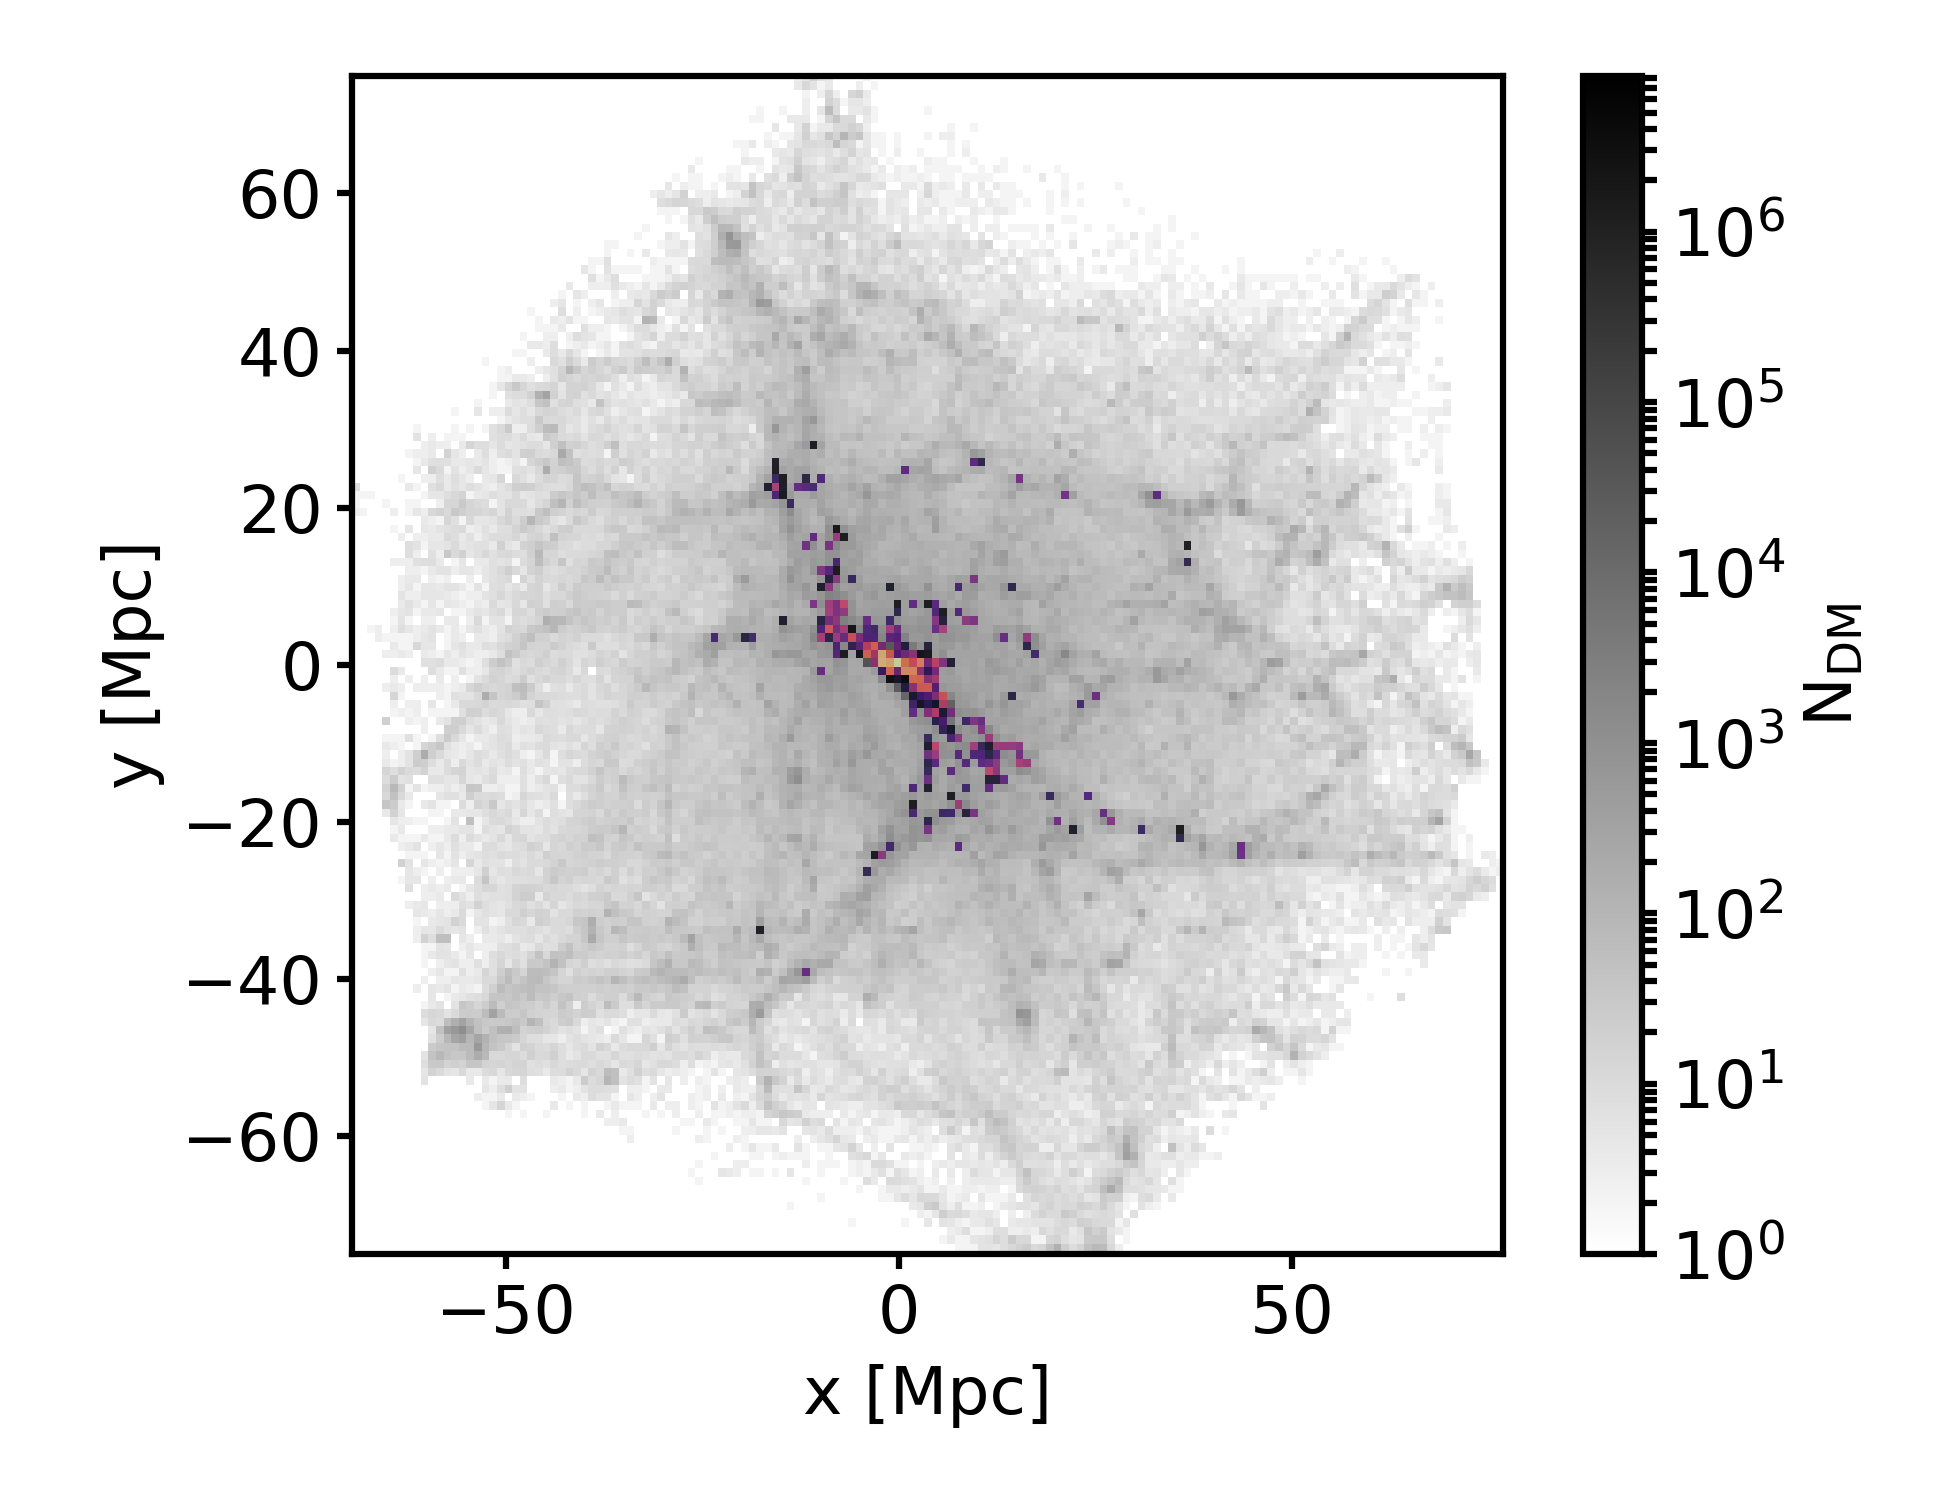
\includegraphics[width=\textwidth]{plots/Auriga/DM_and_stars_xy_distribution.png}
	    \label{fig:DM_stars_xy}
    \end{subfigure}
    
    \begin{subfigure}[b]{0.8\textwidth}
    \centering
    	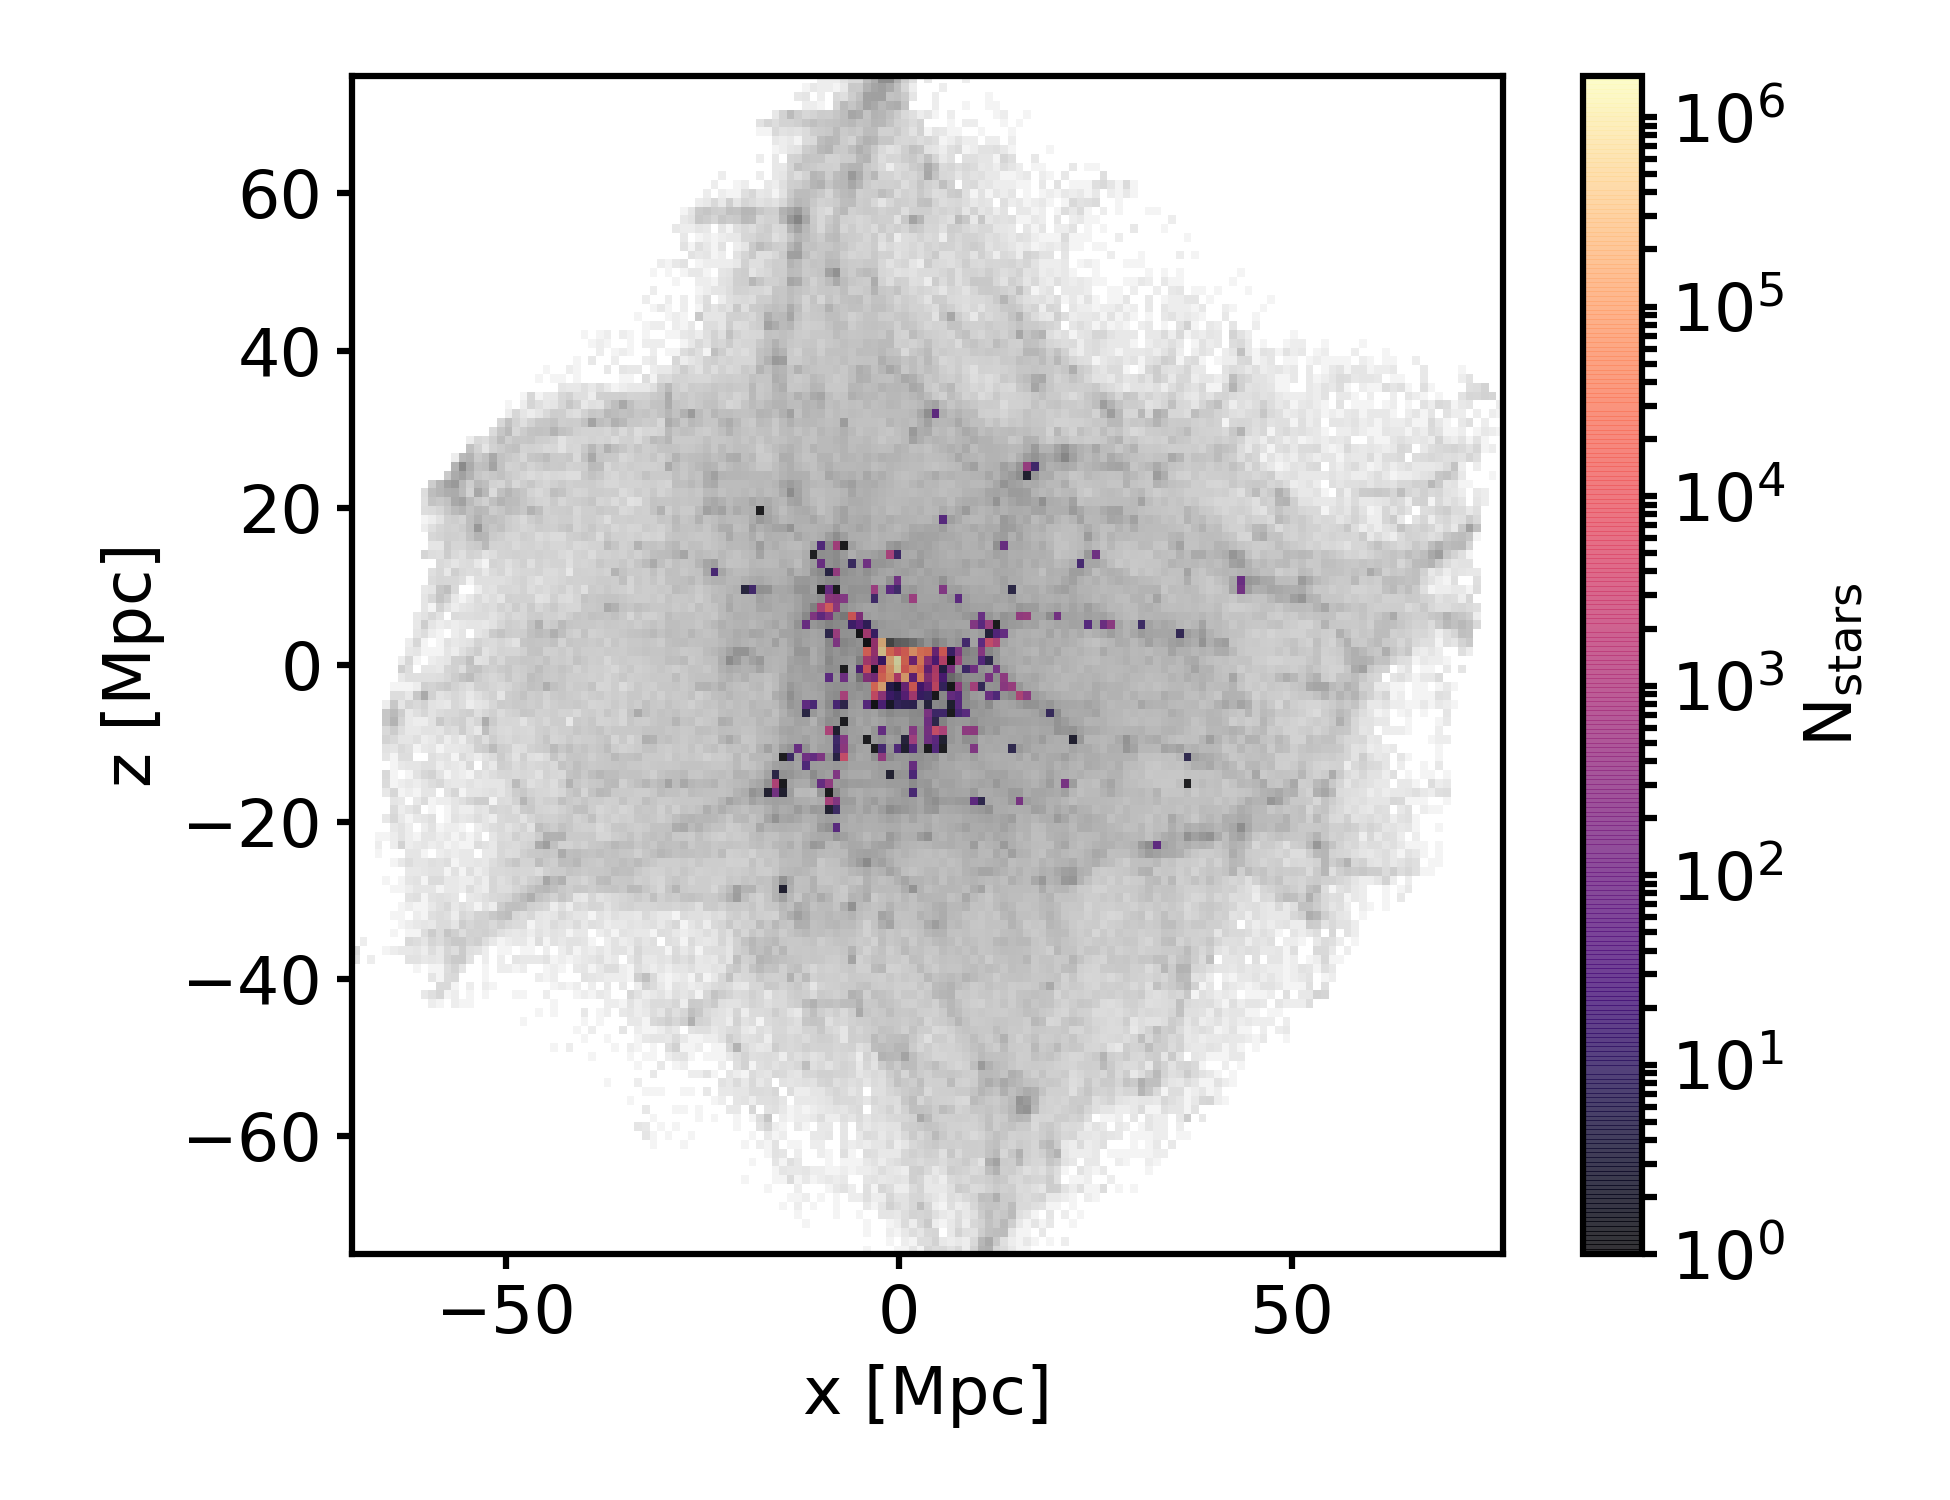
\includegraphics[width=\textwidth]{plots/Auriga/DM_and_stars_xz_distribution.png}
    	\label{fig:DM_stars_xy}
    \end{subfigure}
    \caption{\ac{DM} (grey) and stellar (colors) particle distribution of the whole simulation Auriga24 at $\textit{z}=0$. The \ac{DM} forms the cosmic web, where the mass gathers along its filaments. Baryonic matter also follows these structures. At the most massive parts of the \ac{DM} distribution, the most stellar particles fell in. This structure is typical of hydrodynamical galaxy simulations.}\label{fig:DM_stars_AU24}
\end{figure}
In Figure \ref{fig:DM_stars_AU24}, we show the distribution of \ac{DM} in grey and stars in colors of the whole range of one selected simulated galaxy. The most bound particle is chosen to be the center at $(\mathrm{x,y,z}) = (0,0,0)$. The filaments of the \ac{DM} distribution are clearly visible. The stellar particles settle along these filaments and clump around the highest \ac{DM} structures. 

\subsubsection{Auriga}\label{subsubsec:auriga_intro}
Auriga is a magnetohydrodynamical zoom-in simulation of an isolated \ac{MW} like galaxy. It is build with AREPO \citep{AREPO} and includes galaxy physics, \ac{AGN} feedback and magnetic fields. Its goal is to match the observables of the \ac{MW} today and to produce its history which can be compared to observations of spiral galaxies in earlier stages of development. All 30 galaxies are run in normal resolution and 3 selected are run in low and high resolution as well. It is consistent over these three resolution levels and therefore do not rely on numerical parameters but only on physical. Auriga is one of the first simulations where this is accomplished. The snapshots go from redshift 127, which is close to the beginning of the universe, to redshift 0, today.  At redshift = 0, different galaxy shapes are evolved. Most of them are spirals but a few are in a merger process. All galaxies have a rich merger history. \citep{AurigaGrand} finds that many properties of the \ac{MW} and \ac{MW} like external galaxies are reproduced by these simulations, such as the mass distribution and the circularity distribution. Others are found to be matching within certain limits, such as the SFR–stellar mass relation matches for low redshift $z<1$ but still results in consistent present-day metallicities, mean stellar ages and colours. The set-up and the results of this set of simulations make Auriga one of the most advanced and comprehensive magneto-hydrodynamical galaxy simulations and a very fruitful sample to carry out our investigations. \\
\begin{figure}[htbp]
\captionsetup{format=plain}
    \centering
    \begin{subfigure}[b]{0.8\textwidth}
	    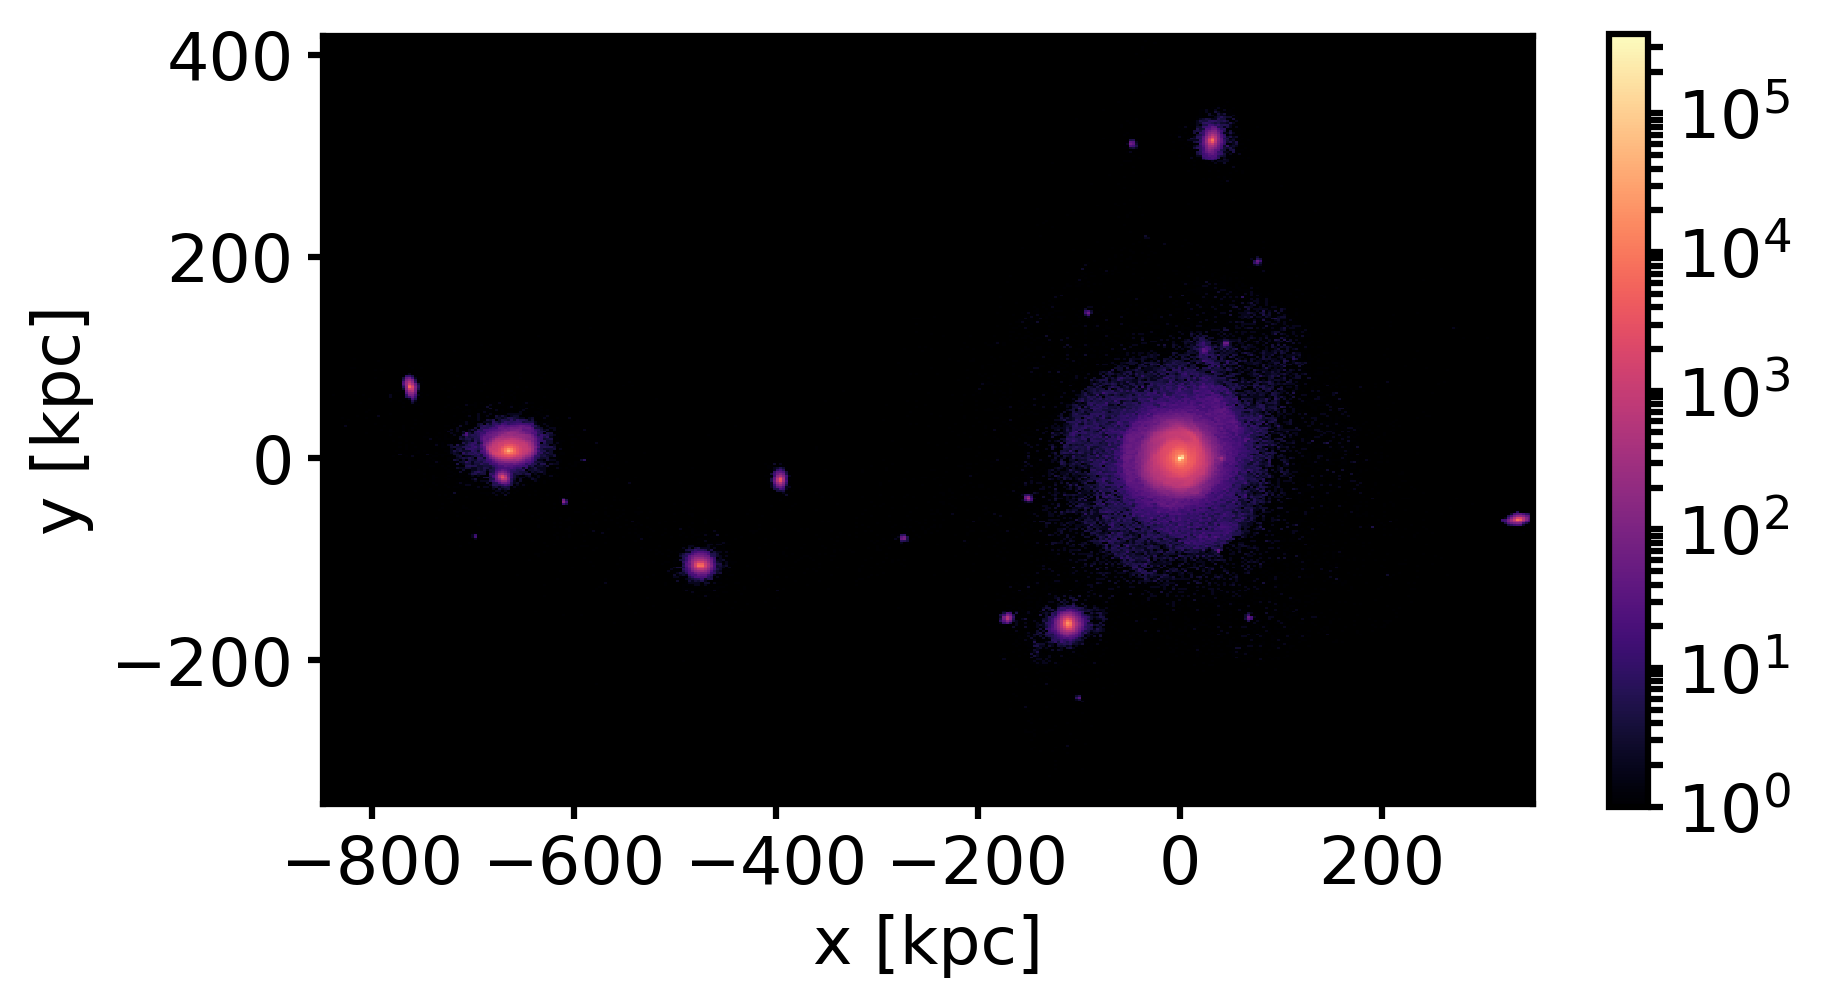
\includegraphics[width=\textwidth]{plots/Auriga/Au24_stars_xy_distribution_halo0.png}
	    \label{fig:Au24_stars_xy}
    \end{subfigure}
    
    \begin{subfigure}[b]{0.8\textwidth}
    \centering
    	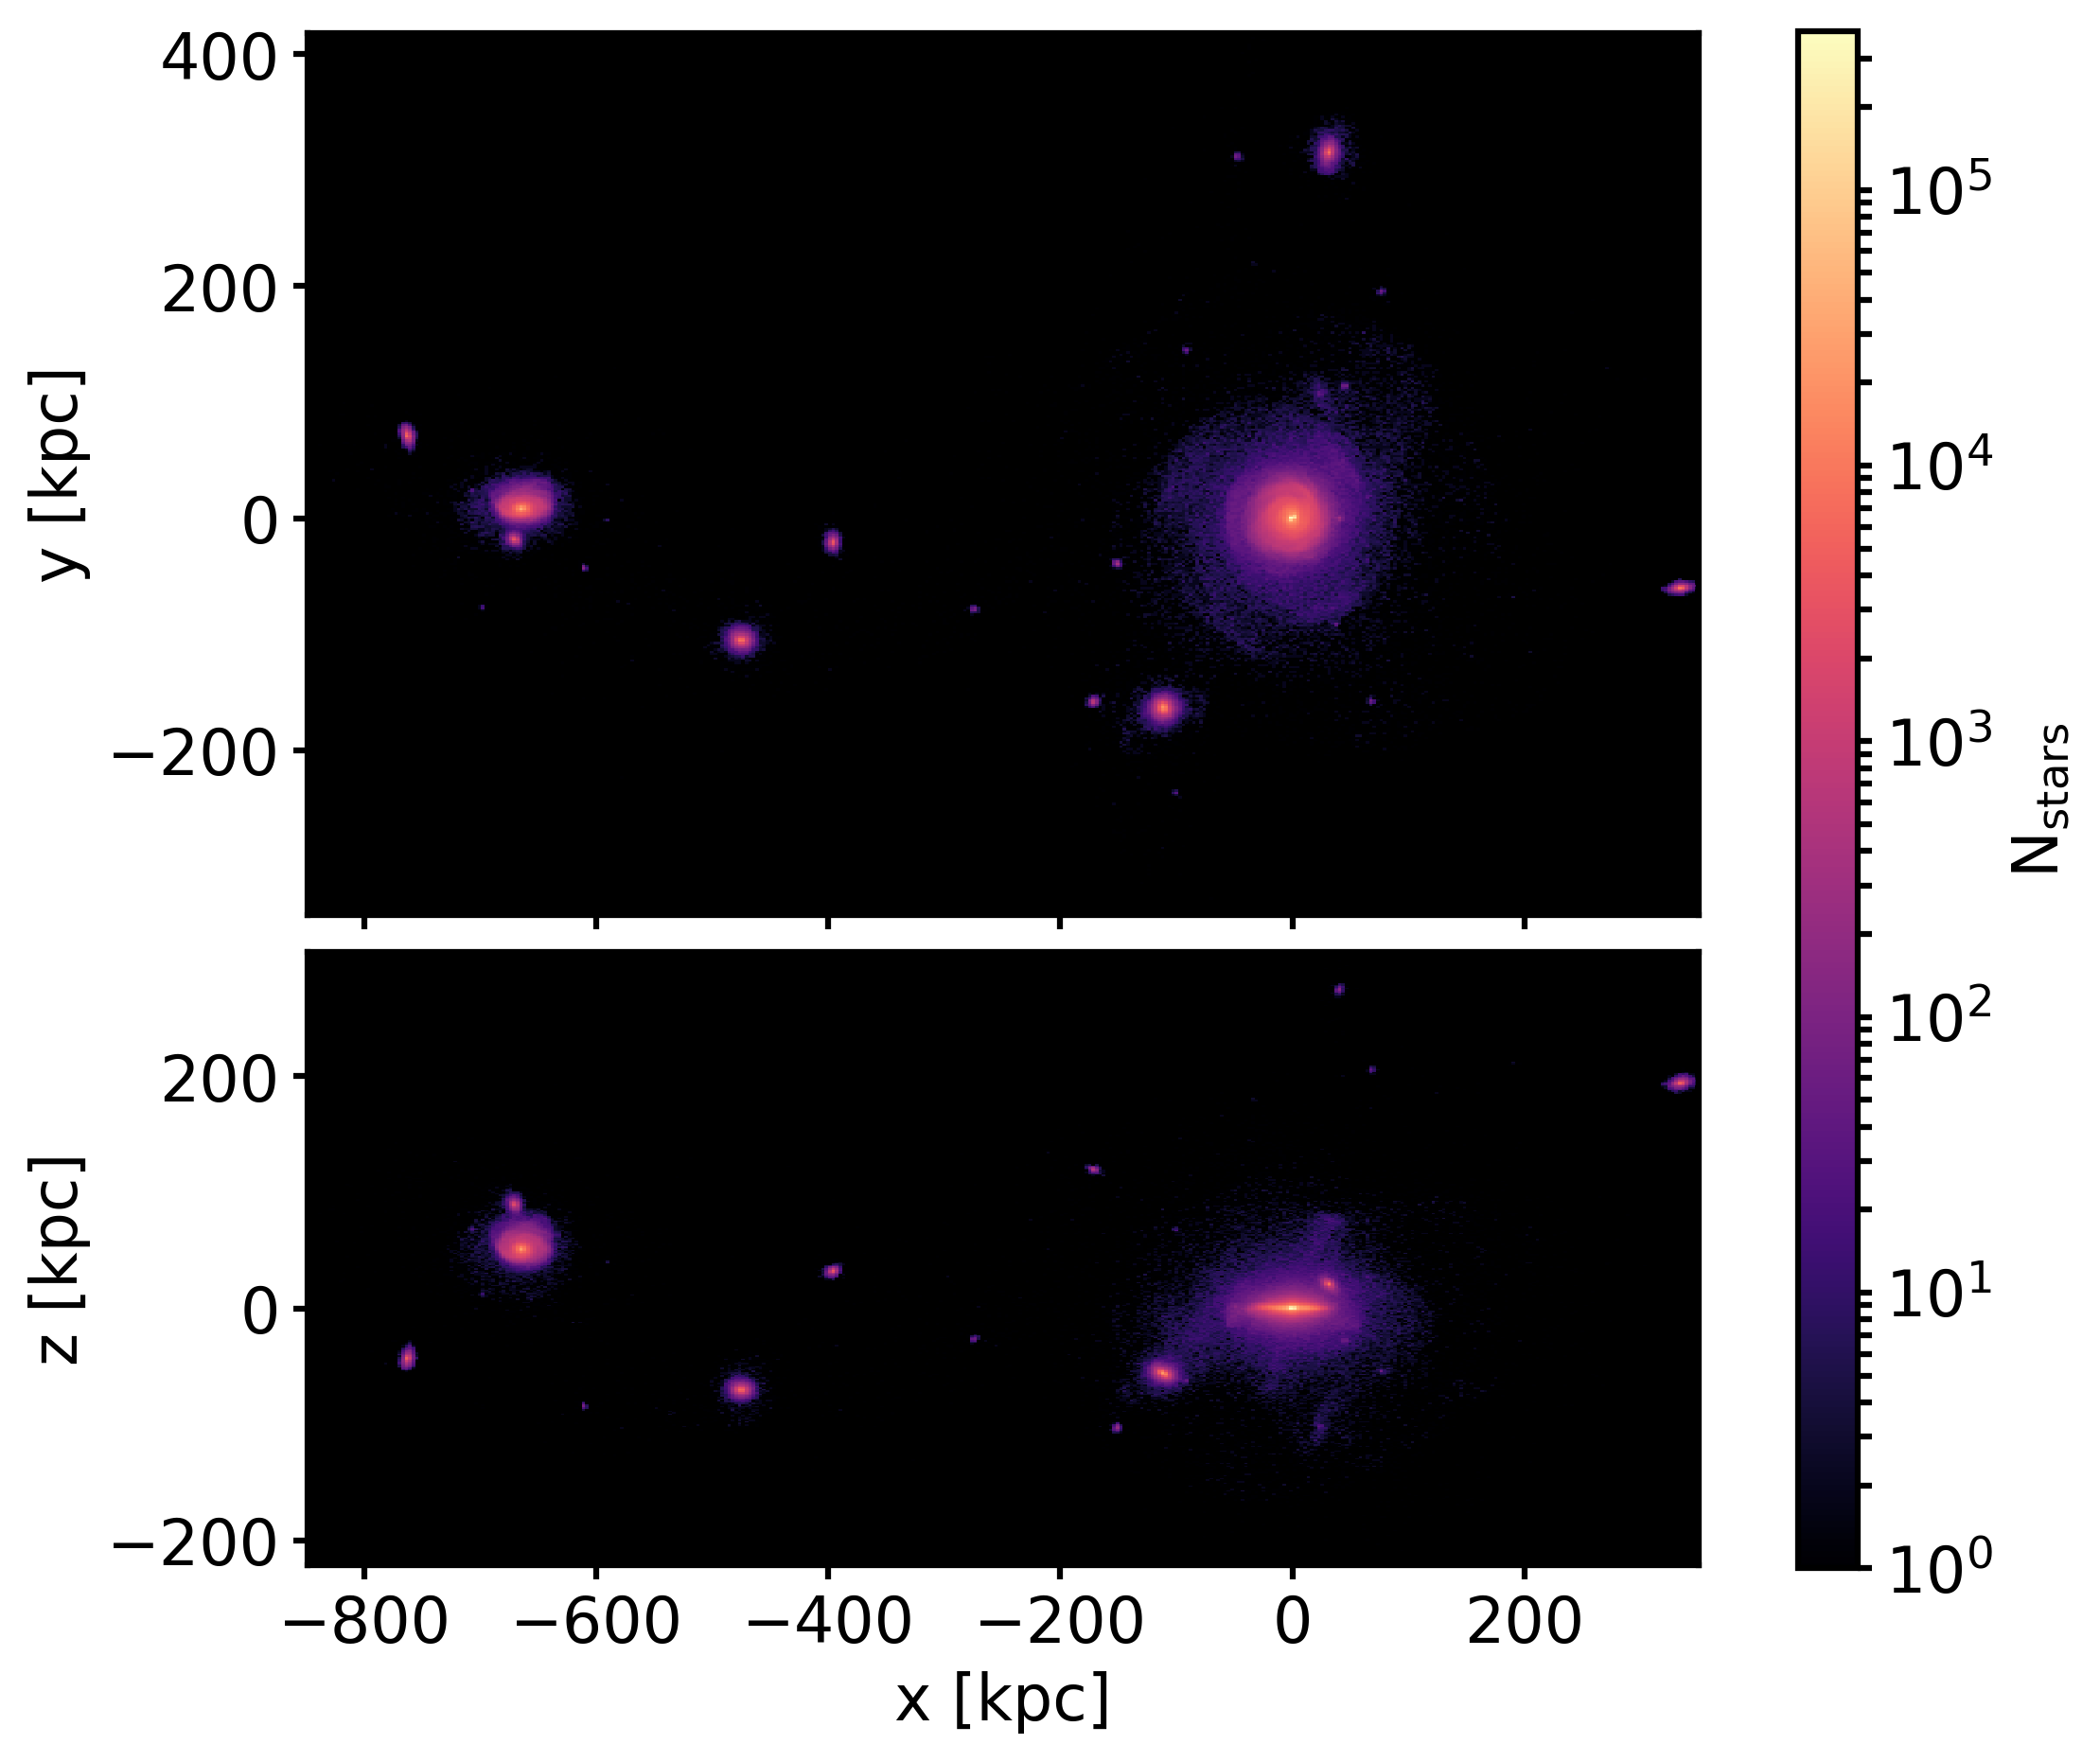
\includegraphics[width=\textwidth]{plots/Auriga/Au24_stars_xz_distribution_halo0.png}
    	\label{fig:Au24_stars_xz}
    \end{subfigure}
    \caption{Stellar distribution of 0th halo at $\textit{z}=0$. The main galaxy is centered at (0,0,0). There are many \acp{DG} around the main galaxy which will eventually merge with it. In the evolution of the simulations, this galaxy has build up mass by merging with \acp{DG}. This mass build up is assumed for and observed in real galaxies.}\label{fig:Stars_AU24}
\end{figure}
\\In Figure \ref{fig:Stars_AU24}, we present the distribution of stellar particles in x-y and x-z direction of the main galaxy and its associated \ac{DG} at redshift $z=0$. Over the course of time, many \ac{DG} already merged with the main galaxy. These make up some of the galaxy's mass and the remnants of these mergers are investigated in Section \ref{sec:Dynamics}.\\
\begin{figure}[htbp]
\captionsetup{format=plain}
    \centering
    \begin{subfigure}[b]{0.8\textwidth}
	    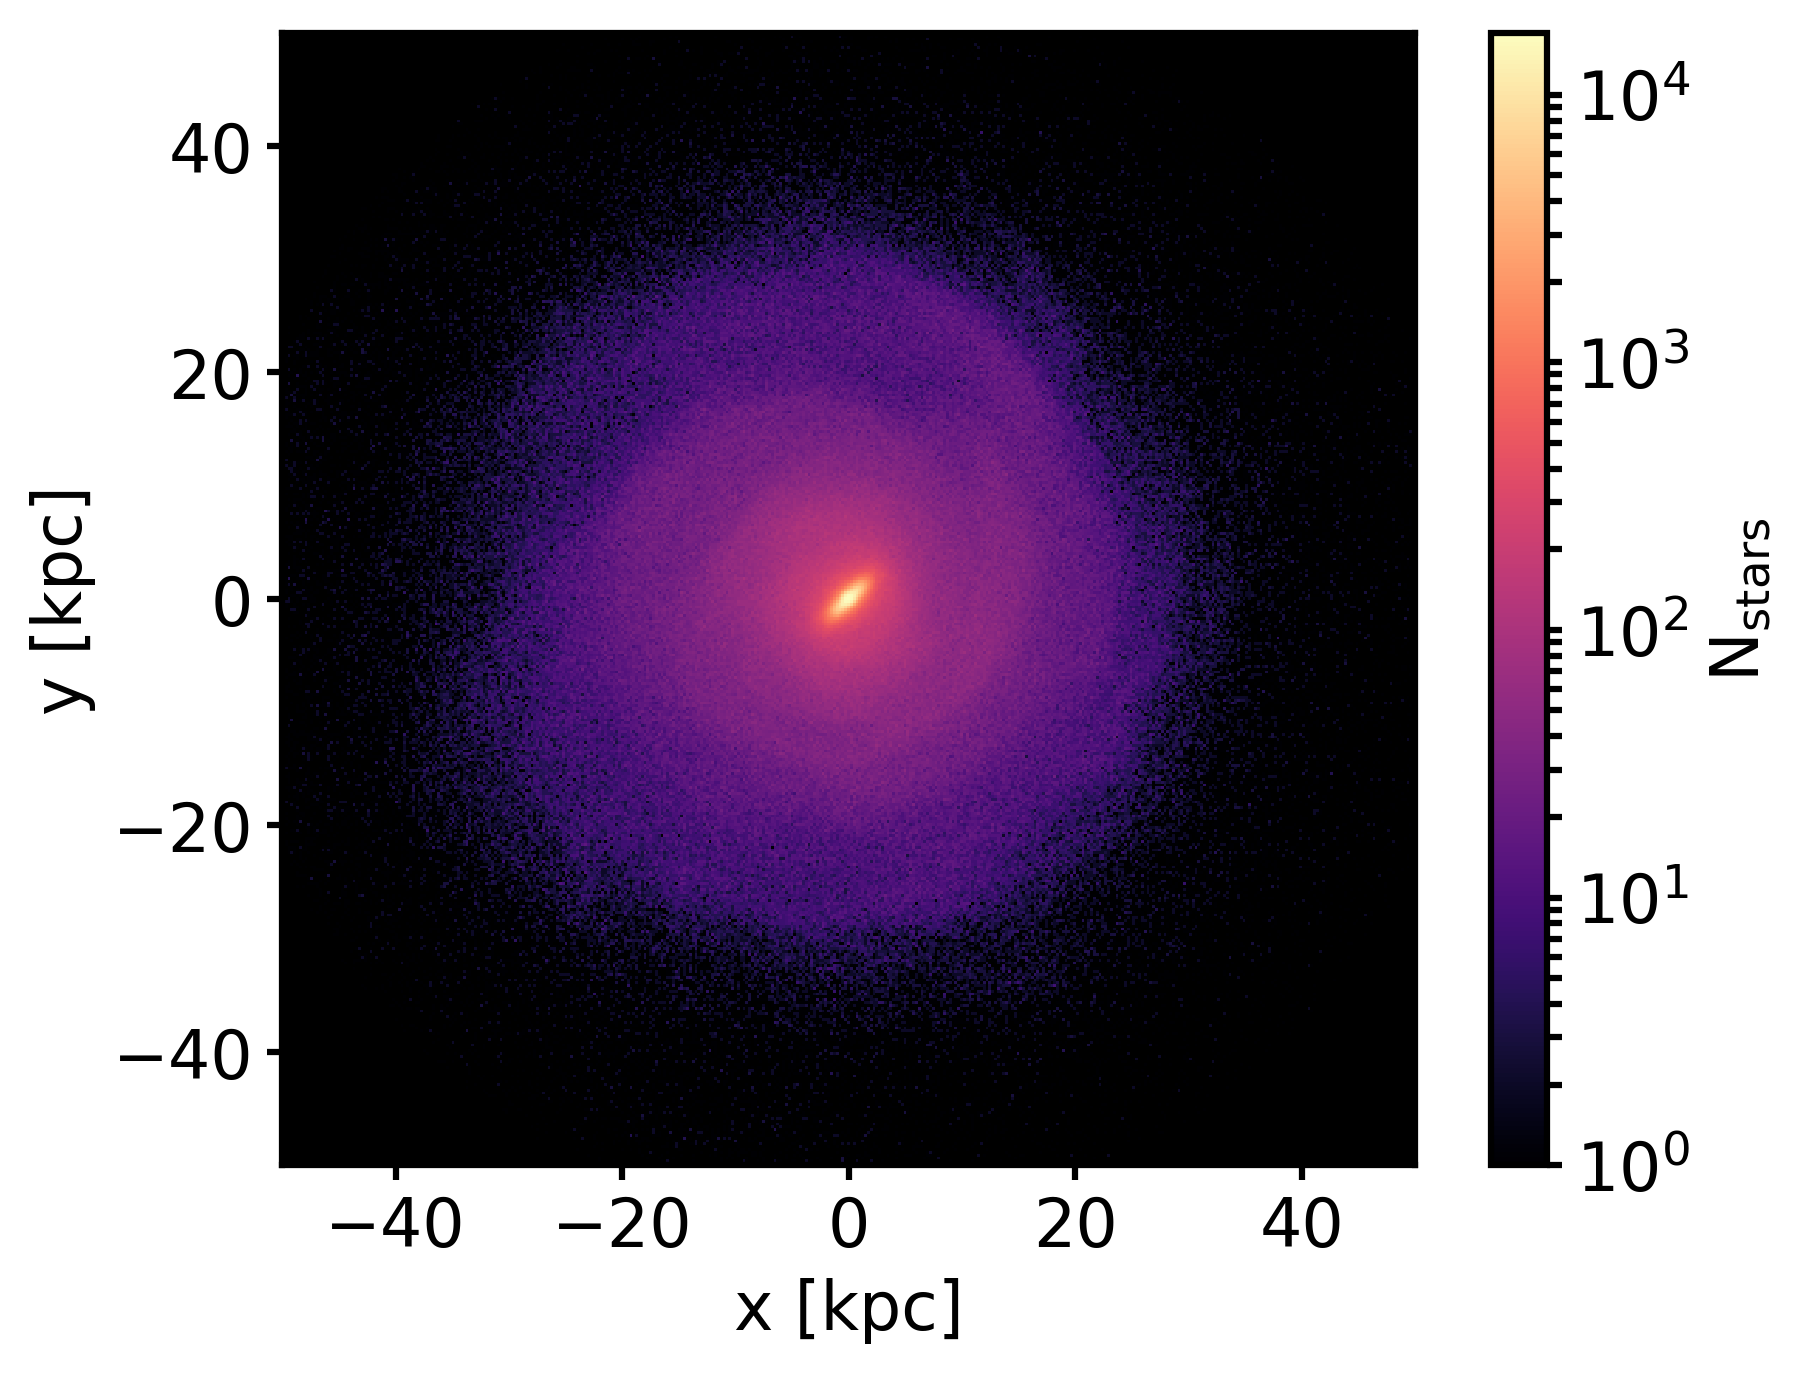
\includegraphics[width=\textwidth]{plots/Auriga/Au24_stars_xy_distribution_halo0_zoomin.png}
	    \label{fig:Au24_stars_xy_zoomin}
    \end{subfigure}
    
    \begin{subfigure}[b]{0.8\textwidth}
    \centering
    	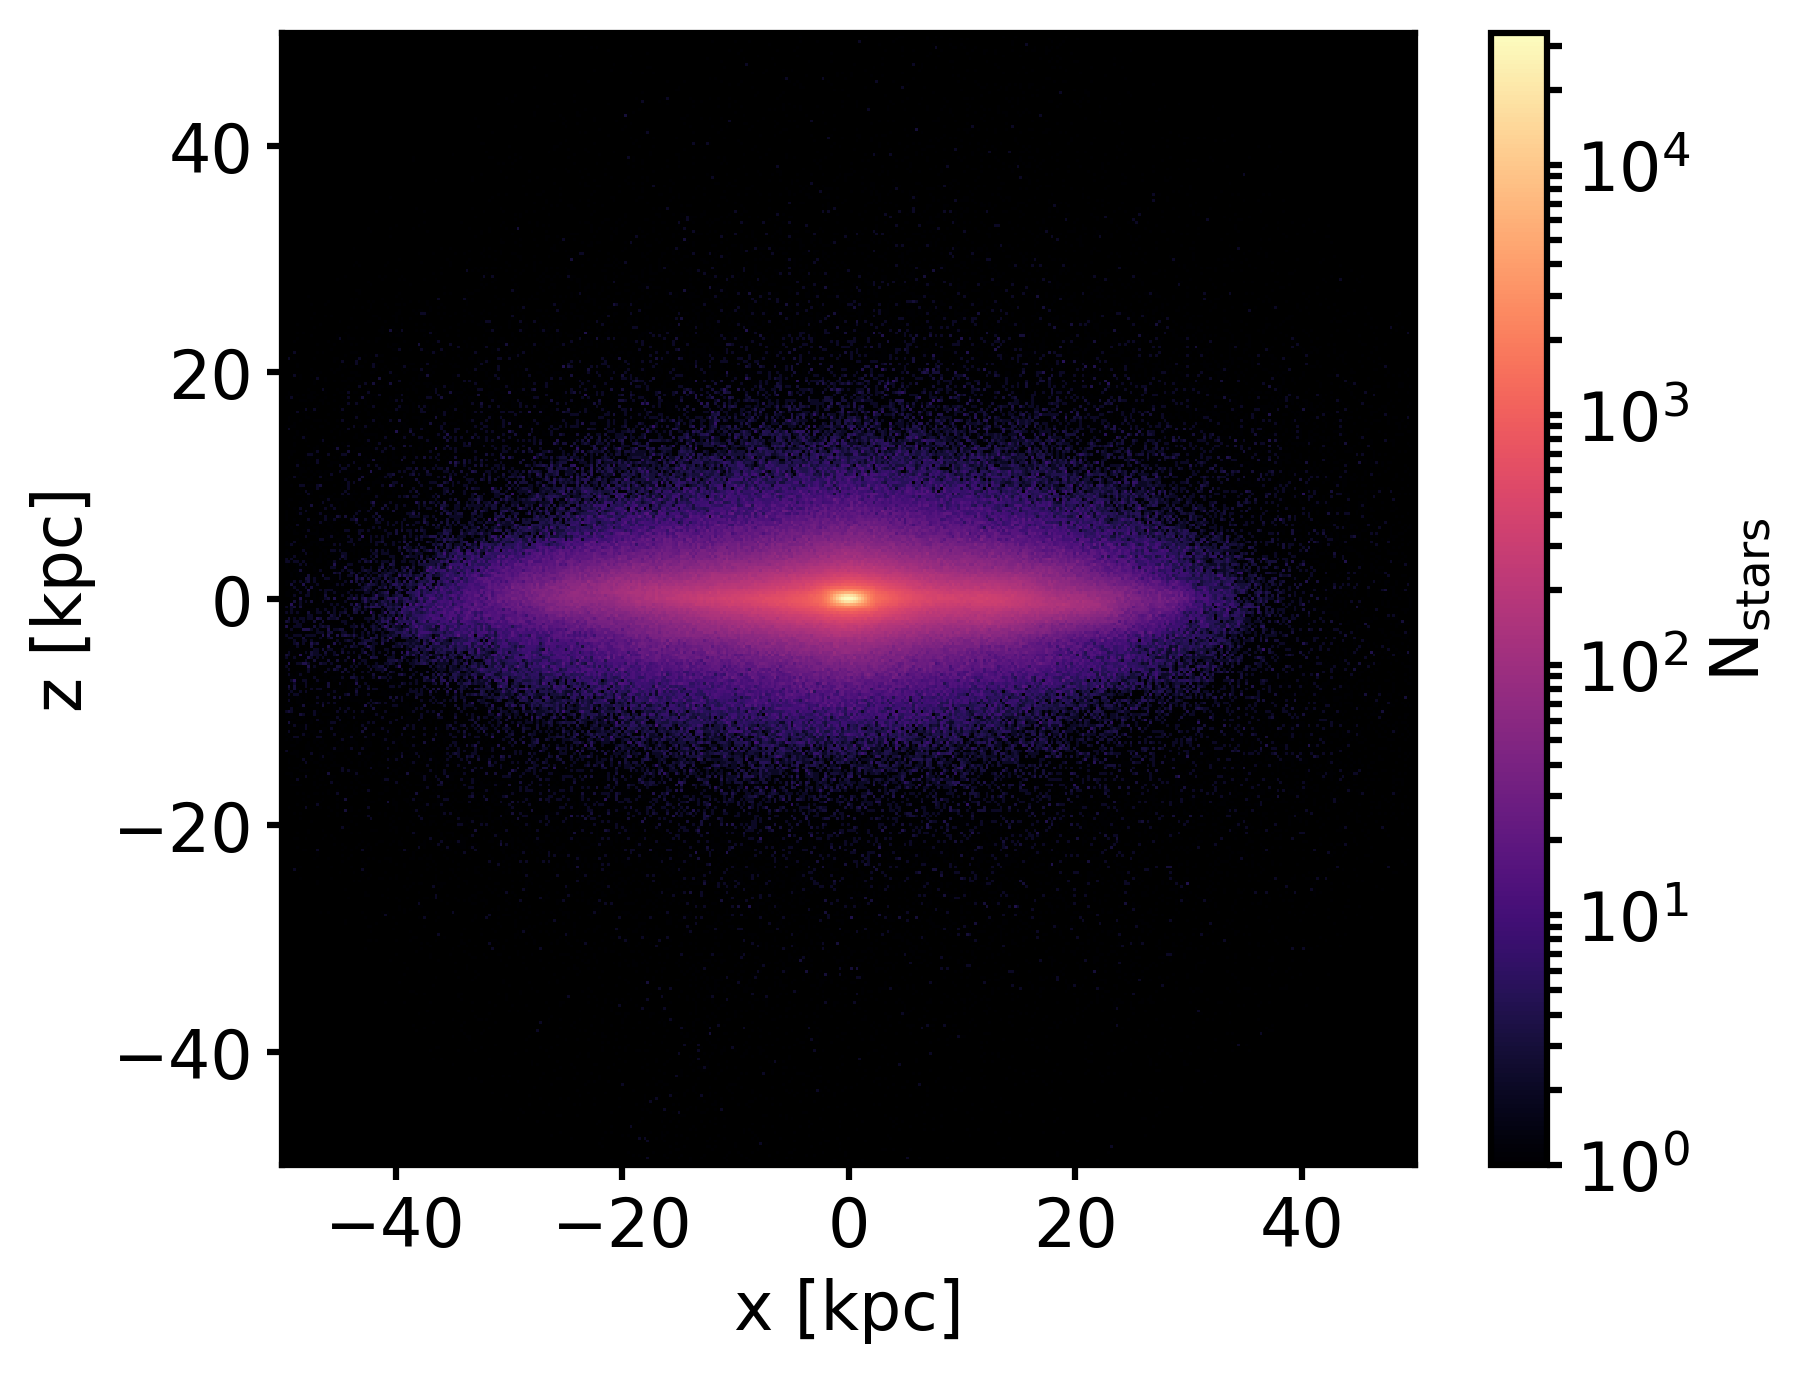
\includegraphics[width=\textwidth]{plots/Auriga/Au24_stars_xz_distribution_halo0_zoomin.png}
    	\label{fig:Au24_stars_xz_zoomin}
    \end{subfigure}
    \caption{Stellar distribution of main galaxy at $\textit{z}=0$. In the upper panel, the galaxy is seen face-on. There, the presence of non-axisymmetric substructure such as spiral arms and a bar is visible. In the lower panel it seen is edge-on. Disk and bulge are clearly present and a close \ac{DG} is visible.}\label{fig:Stars_AU24_zoomin}
\end{figure}
\\A face-on and edge-on view of the main galaxy is presented in Figure \ref{fig:Stars_AU24_zoomin}. We can see axisymmetric features such as bulge and disk and clear non-axisymmetric features such as a bar and spiral arms. This galaxy resembles the \ac{MW} and other late-type galaxies.
\subsection{Best fit potential}\label{subsec:best_fit_pot}
The best fit potential of a galaxy should be a analytic, axisymmetric potential so that we are able  to compare our results to the results of observers, since they mostly fit external galaxies in such a structure. We need to take into account that the galaxy evolved not isolated but went through many mergers and therefore its potential is either analytic nor axisymmetric but has a lot of substructure. The fit is only a vague approximation. Also it is self-consistent so changes in potential influence the velocities of the objects inside and changes on the positions of the objects will change the gravitational potential. Since we fit a potential to each snapshot we have a time-dependent potential. The routine and results in this Section are for the $z=0$ snapshot but the same routine was applied for all snapshots since a lookback time of \SI{10.5}{Gyr}. We also need to include a disk and bulge decomposition which is not natural in a cosmological simulation. As the gas evolves in cells, we cannot calculate its density easily. Therefore, we do not consider it in our potential fits. Since we want to recreate observers way of looking at galaxies we do not need to include gas as observers in e.g. \ac{MGE} fits \citep{MGE...Monnet, MGE...Emsellem} also only take stellar light into account. 
\\The potentials we fit and use as well as the action calculation routines are implemented in galpy \citep{Bovy...galpy...2015}.

\subsubsection{galpy}\label{subsubsec:galpy}
galpy is a well tested and well documented python package for galactic dynamics. It includes analytic spherical, axisymmetric and ellipsoidal triaxial potentials and fast routines, additionally implemented in C, for the calculation of orbits, action-angles and \acp{DF}. galpy has its own internal units which has to be considered and understood before using it.
\\In this work, we first fit a set of analytic potentials from to the simulation which is described in the remainder of this Section. Then, we calculate actions of accreted \acp{GC} in a variety of potentials in galpy and investigate the results in the next Section. 

\subsubsection{Component decomposition}\label{subsubsec:decomp}
To fit a potential to each component, we first need to decompose the different parts. We assume that all \ac{DM} particles belonging to the main galaxy make up its halo. The stellar particles belong to either the spheroid or the disk. We distinguish these components by the use of the circularity parameter 
\begin{equation}
    \epsilon = \frac{L_z}{L_{z,max}(E)}
\end{equation}
where $L_{z,max}(E)$ is the maximum angular momentum allowed for the orbital energy $E$. 
$\epsilon = 1$ is a prograde circular orbit in the disc plane. $\epsilon = -1$ is a retrograde circular orbit in the disc plane. $\epsilon \sim 0$ is an orbit with a very low $z$-component of angular momentum which may be highly inclined to the disc spin axis and/or be highly eccentric.  

\cite{AurigaGrand} uses two different methods two distinguish the components and to get their mass ratio:
\begin{enumerate}
\item Under the assumption, that the bulge has zero net rotation, mirror negative $\epsilon$ as bulge material, the rest belongs to the disk.
\item All particles with $\epsilon > const$ are assigned to the disk, where $const = 0.7$ is set heuristically.
\end{enumerate}

\cite{AurigaGrand} find that the first method generally overestimates the \ac{D/T} ratio while the second approach underestimates it by choosing only kinematically very cold particles. Since we do not only want to get the mass ratio of \ac{D/T} but also want to tag each particle clearly, we use the second method. Nevertheless, the true assignment lies somewhere between these method. 

\begin{SCfigure}%[htbp]
\captionsetup{format=plain}
    \centering
    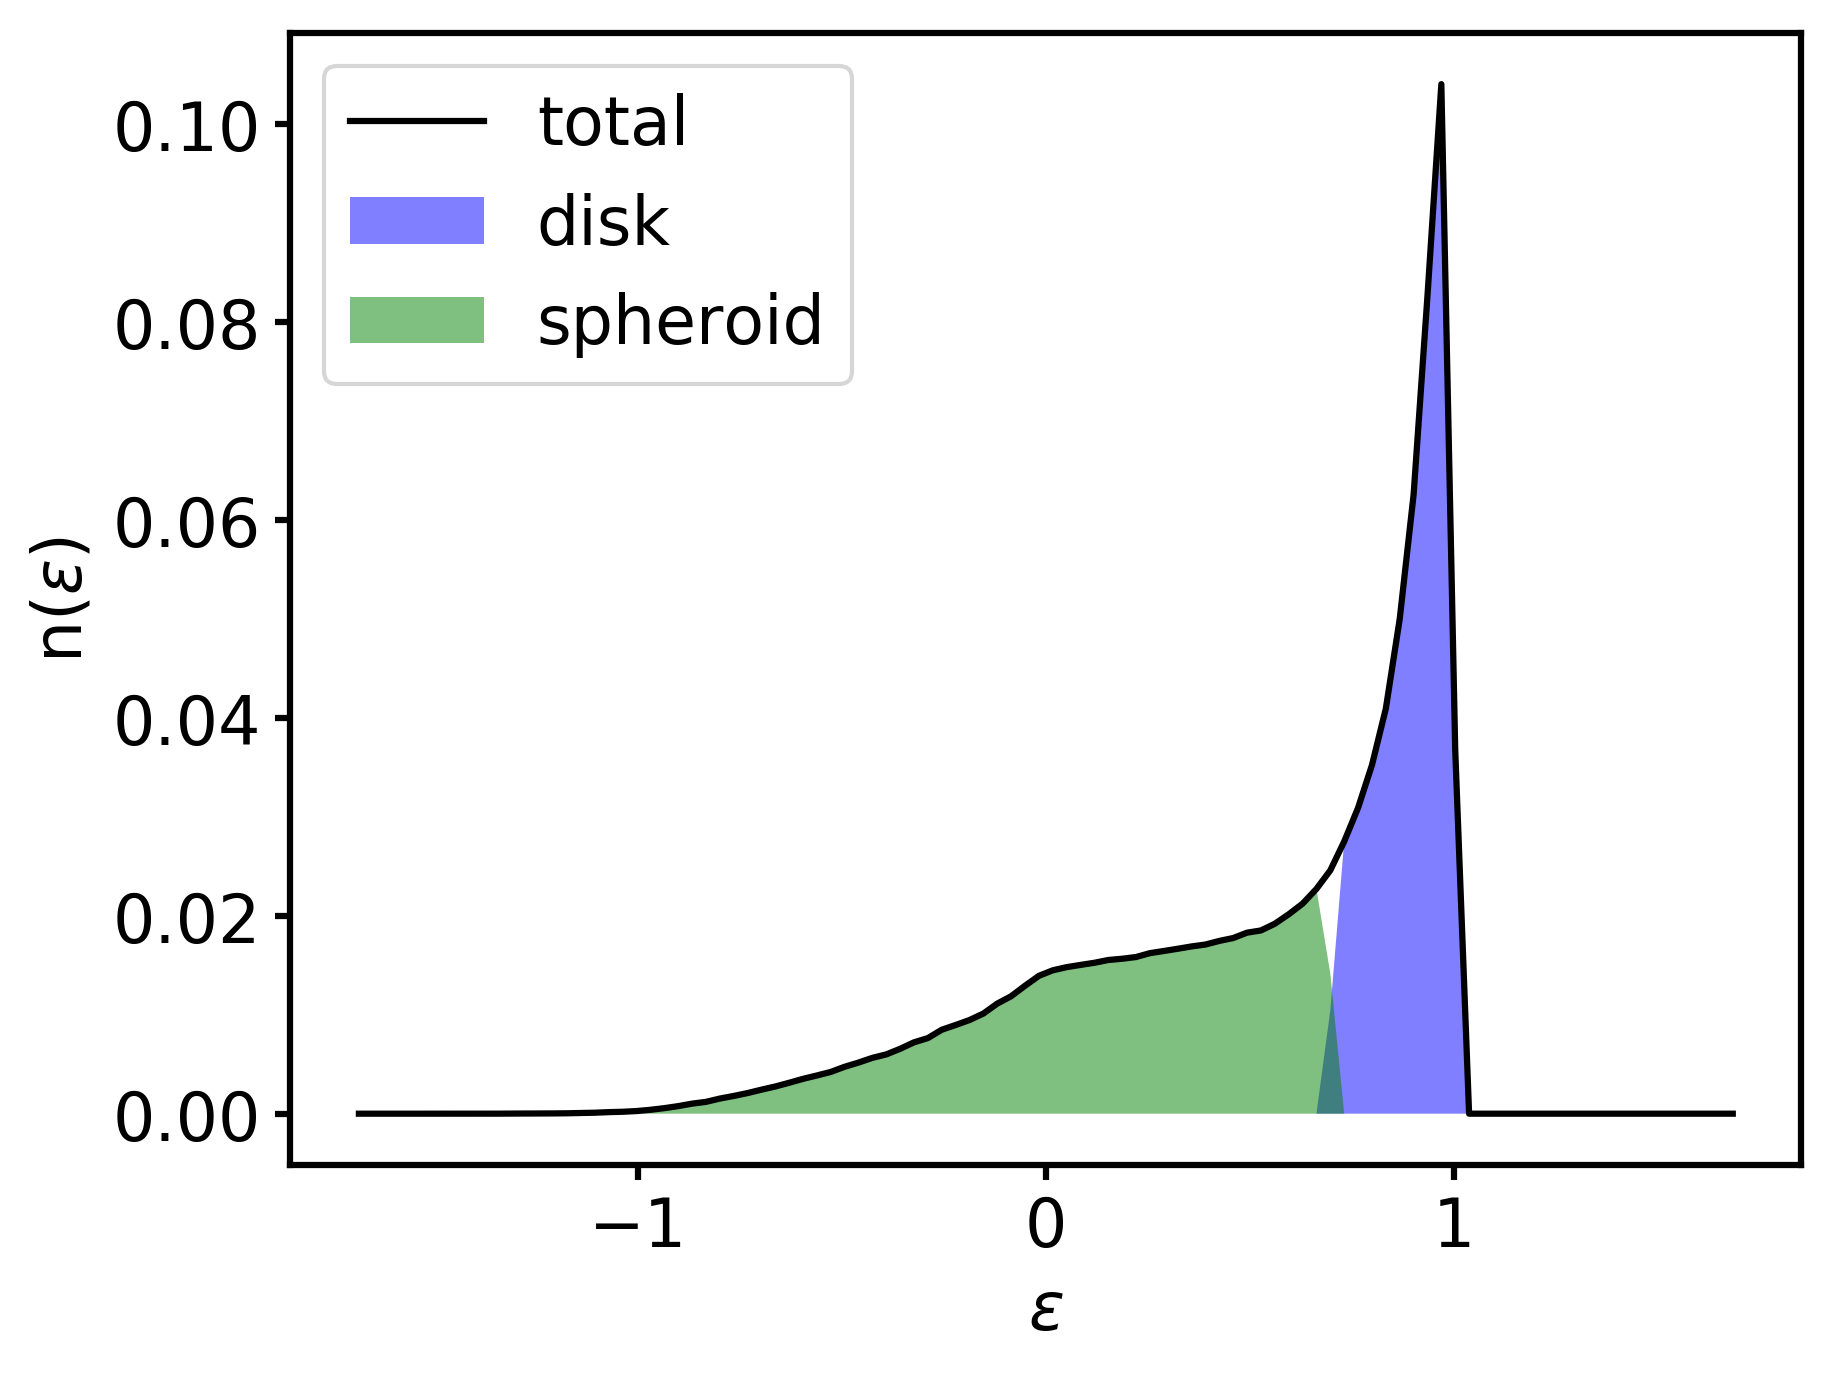
\includegraphics[width=0.6\textwidth]{plots/Auriga/decomposition_snap_127.png}
\caption{Decomposition of stellar disk and spheroid by their circularity. It was carried out for all stellar particles within the galaxy radius. The black line represents the total circularity. The green area is the the spheroid component and the blue is the disk component. The disk particles were selected by having a circularity above 0.7. The disk to total number ratio is 0.47.}\label{fig:decomposition}
\end{SCfigure}
\\In Figure \ref{fig:decomposition}, we show a histogram of the circularity with our decomposition. The blue part is the disk portion while the yellow part is the spheroid. Together they add up to the black solid line, the total number. The \ac{D/T} ratio is 0.47.
Since we can assign the particles to be in the spheroid or disk easily, we use this composition to find the disk and spheroid where we fit our potential to. 


\subsubsection{Disk potential}\label{subsubsec:disk_pot}
We fit the disk with a \citet{MNprofile} potential following the profile 
\begin{equation}
\Phi(R,z) = -\frac{GM}{\sqrt{R^2+(a+\sqrt{z^2+b^2})^2}}
\end{equation} 
with scale length $a$ and scale height $b$ which provides a disk with a finite thickness. If $b\rightarrow 0$, the disk will be infinite thin and if $a \rightarrow 0$ the potential has a spherical density distribution. $b/a$ therefore defines the flattening of the system. It is a rather simply model with only a small computational costs. Therefore it is widely used. It has limitations in the mid-plane ($z=0$) at high $R$. 
\\To fit the disk potential, we bin the stellar disk in $(R, z)$ and calculate the density of each bin. Then, we fit the \ac{MN} density to the data using the scipy \citep{scipy....2001} routine optimize.curve\_fit. For the \ac{MN} potential, we have the scale length a$_{\mathrm{MND}}$, the scale height b$_{\mathrm{MND}}$ and the contribution to the total circular velocity v$_{0, \mathrm{MND}}$ as fit parameters. The best fit parameters are listed in Table \ref{tab:pot_best_fit_params}.
\begin{figure}[htbp]
\captionsetup{format=plain}
    \centering
    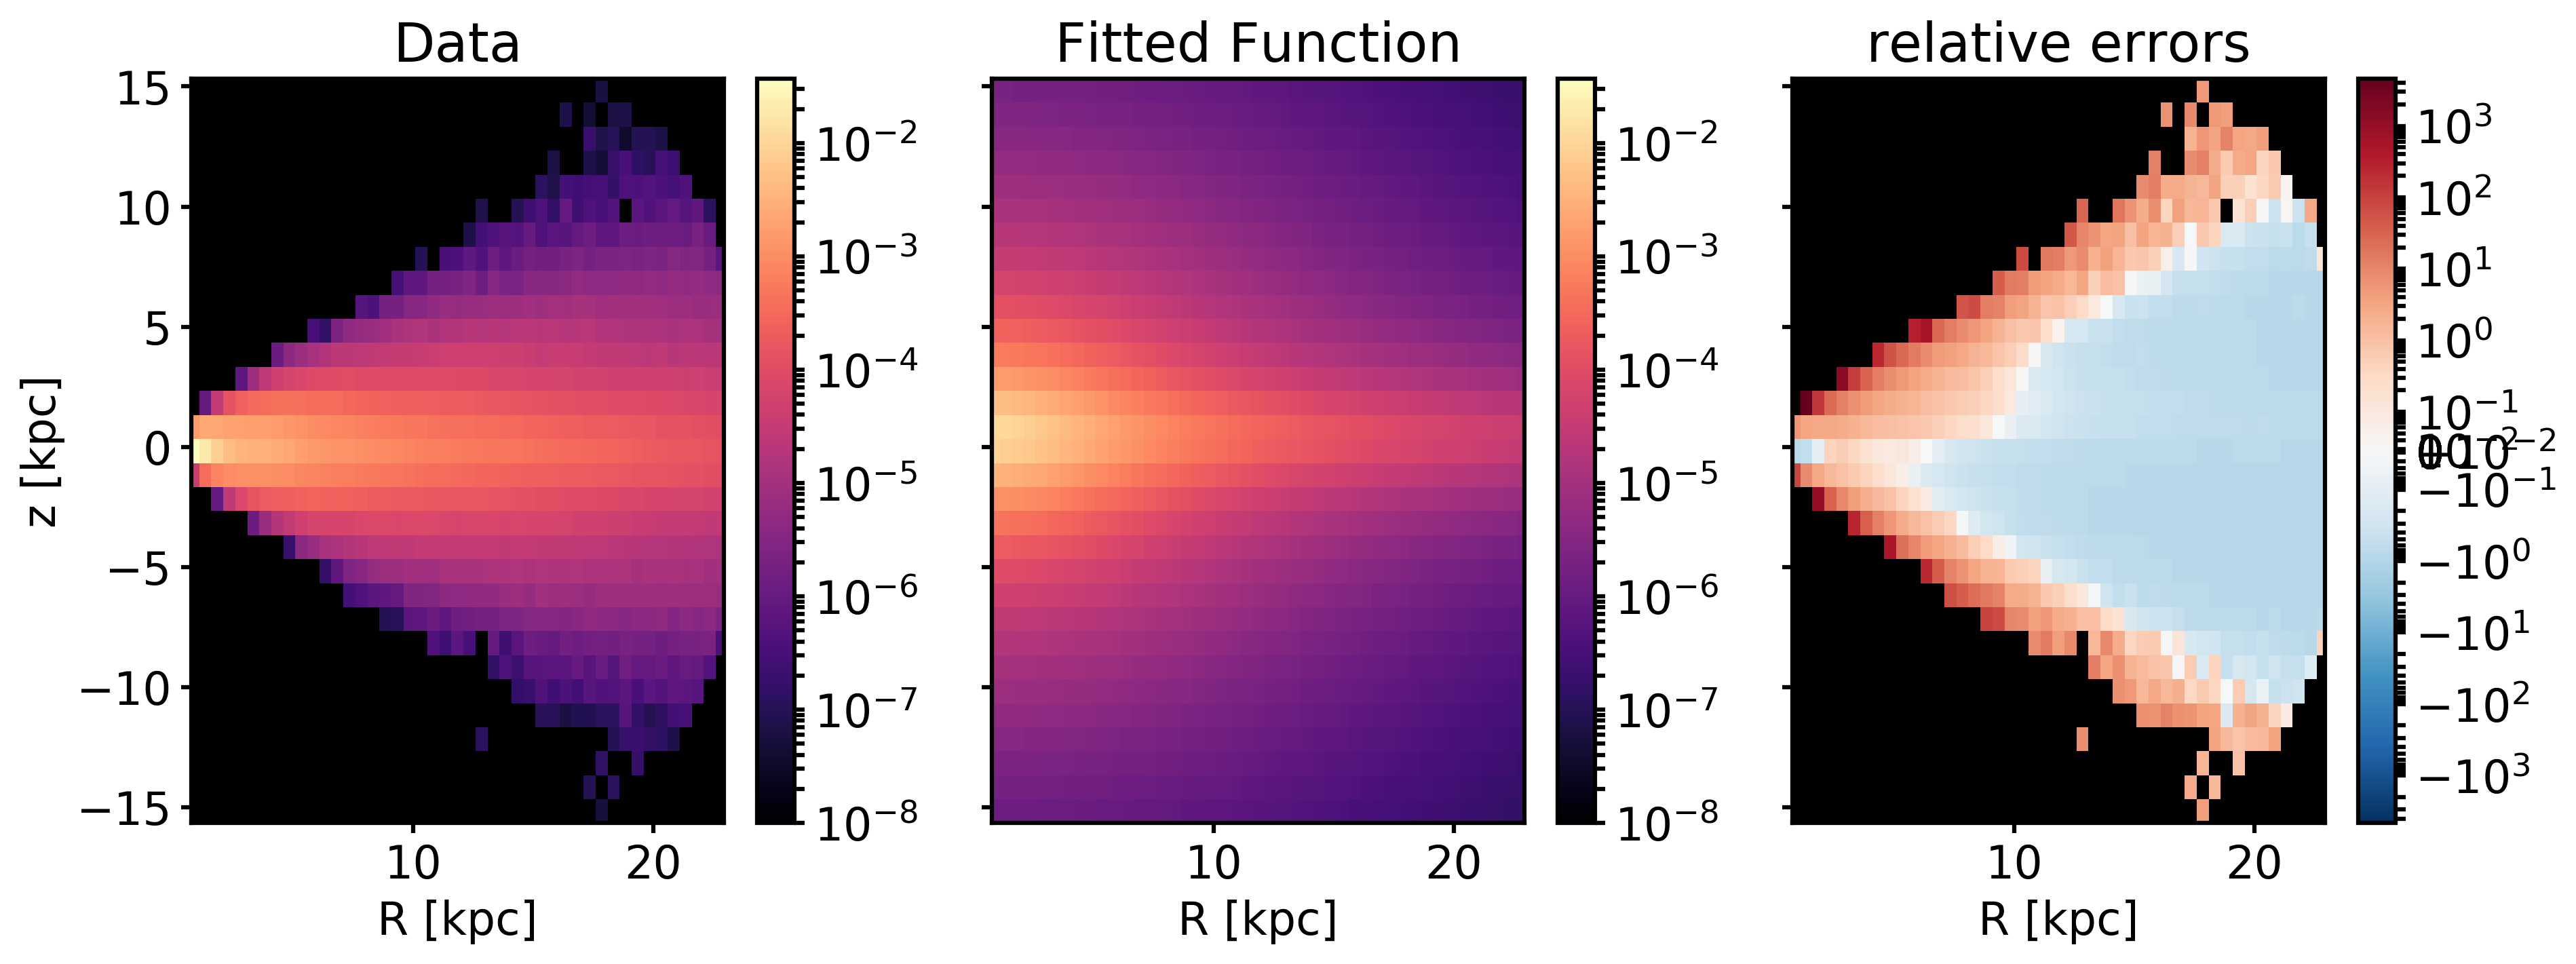
\includegraphics[width = \textwidth]{plots/Auriga/MND_best_fit_snap_127.png}
    \caption{Density fit of the \ac{MN} profile to the disk. \textit{Left panel:} in $(R,z)$ binned mass density of the simulation data. \textit{Middle panel:} in $(R,z)$ binned mass density of the best fit \ac{MN} profile. \textit{Right panel:} relative errors \(\Delta_\rho = (\rho_{\mathrm{fit}}- \rho_{\mathrm{data}})/\rho_{\mathrm{data}}\) of the best fit.}
    \label{fig:MND}
\end{figure}
\\The best fit is shown in Figure \ref{fig:MND}. In the left panel, we see the binned data. Due to the kinematic selection of disk particles, we see that the disk exceeds the height of a typical disk in a spiral galaxy. This is negligible since the density falls off quickly above an absolute height of \SI{1.5}{kpc}. At the black parts of the histogram, there was no data. Therefore, they weights of the fit lay on the actual disk. In the middle panel, we show the binned density of the best fit \ac{MN} profile. We can clearly see the disk. Since it is an analytic potential, the density can be calculated for every bin in $(R, z)$. In the right panel, the relative errors \(\Delta_\rho = (\rho_{\mathrm{fit}}- \rho_{\mathrm{data}})/\rho_{\mathrm{data}}\) are plotted. In the edges of the data, these errors are very high. This is most probably due to selection effects and cutting the data there while the fitted density is still smooth there. In the disk and outer regions, the relative error is very small (\(<1\)). Due to these small errors, we are confident that this is the best fit of the analytic \ac{MN} potential to the non-analytic and selected-through-decomposition disk. 


\subsubsection{Spheroid potential}\label{subsubsec:spher_pot}
For the central stellar spheroid, we apply a \citet{Hernquistprofile} potential which has the density 
\begin{equation}
    \rho = \frac{M}{2\pi}\frac{a}{r}\frac{1}{(r+a)^3}
\end{equation}
where $M$ is the stellar mass of the spheroid and $a$ is its scale length. It has a gentle power-law cusp and at large radii, it declines like $r^{-4}$. \citet{Hernquistprofile} has shown that it reproduces properties of elliptical galaxies and spherical bulges. 
\\
\begin{SCfigure}
\captionsetup{format=plain}
    \centering
    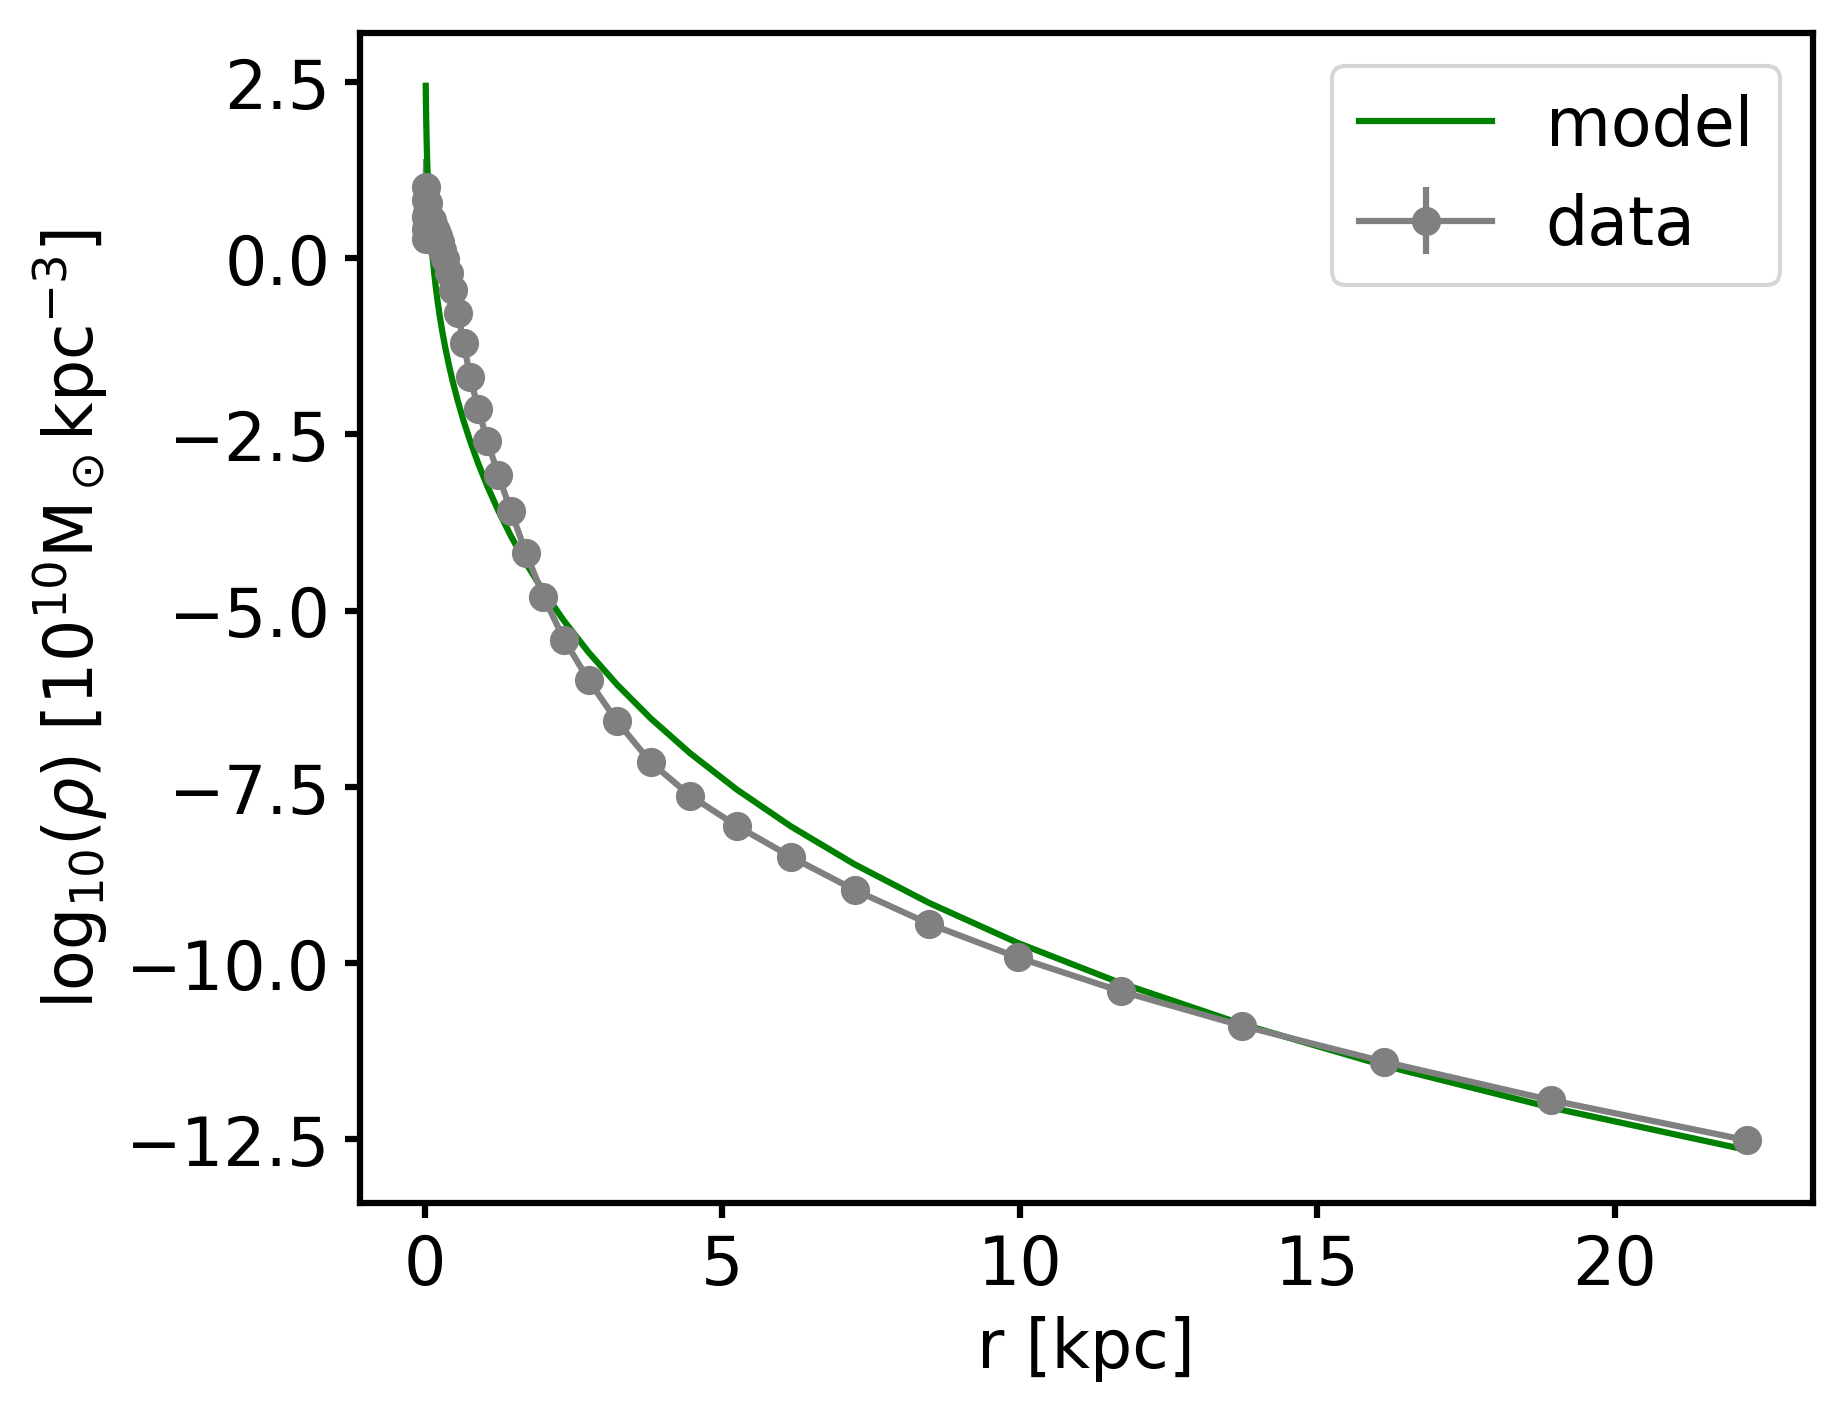
\includegraphics[width=0.7\textwidth]{plots/Auriga/spheroid_density_fit_snap_127.png}
    \caption{Spheroid density: data with errors (grey dots) and best fit (green line). The data is binned logarithmically in r. Their standard deviation is too small to be seen. In the inner part, r $<10$kpc, the density is both under and over estimated. In the outer parts, the fit matches the data.}
    \label{fig:spheroid_fit}
\end{SCfigure}
\\Since the Hernquist density is spherical symmetric, we bin it to logarithmic bins in the radius r. The data and best fit densities are shown in Figure \ref{fig:spheroid_fit}. While in the inner part the fit does not match the data too good, in the outer parts it fits. Since most of the particles we investigate in Section \ref{sec:Dynamics} are more far away from the center than \SI{10}{kpc}, the fit is acceptable to carry out this analysis.

\subsubsection{Halo Potential}\label{subsubsec:halo_pot}
We model the \ac{DM} halo with a \citet{NFWprofile} profile following the formula 
\begin{equation}
    \frac{\rho(r)}{\rho_{crit}} = \frac{\delta_c}{(r/r_s)(1+r/r_s)^2} = \frac{\mathrm{amp}}{4 \pi a^3}\frac{1}{(r/a)(1+r/a)^2}
\end{equation} with scale radius $r_s = a$, the critical density $\rho_{crit} = 3H^2 / 8\pi G $ and a characteristic and dimensionless density $\delta_c$ which can be rewritten as \(\rho_{crit}\cdot\delta_c = \frac{\mathrm{amp}}{4\pi a^3} \). The \ac{NFW} profile is derived from \ac{DM} only hydrodynamical simulations and found to accurately describe \ac{DM} halos. 
\\With the best fit potentials for the stellar components, we set up a potential in galpy with all three components and fit it to the 'pot' value of 100000 randomly selected DM particles using the scipy.optimize.differential\_evolution routine. With that method, we find the best fit scale length of the DM halo, a$_{\mathrm{NFWH}}$as well as the total circular velocity v$_{0,\mathrm{tot}}$ at a given distance R$_0$. From that total circular velocity we can subtract the fraction from the stellar components to get the \ac{DM} component, $v_{0,\mathrm{NFWH}} = \sqrt{v_{0,\mathrm{tot}}^2 - v_{0, \mathrm{MND}}^2 - v_{0, \mathrm{HB}}^2}$. The resulting parameter values are summarized in Table \ref{tab:pot_best_fit_params}. 

\subsubsection{Total potential}\label{subsubsec:tot_pot}
After fitting each component individually, we add them up to get a total potential. In Table \ref{tab:pot_best_fit_params}, we summarize our results for the last snapshot as described in the previous Sections. 

\begin{table}[htbp]
\captionsetup{format=plain}
    \centering
    \begin{tabular}{@{}llll@{}}
         \toprule
         component& potential & parameters \& values &fitting method  \\
         \midrule
         stellar disk& \makecell[tl]{Miyamoto\\-Nagai}&\makecell[tl]{a$_{\mathrm{MND}}$ = \SI{2.97}{kpc}\\b$_{\mathrm{MND}}$ = \SI{1.64}{kpc}\\v$_{0,\mathrm{MND}}$ = \SI{105.00}{km.s^{-1}}} & \makecell[tl]{\ac{MN} density fitted \\to density bins \\of disk in $(R,z)$.}\vspace{3mm}\\
         %\midrule
         \makecell[tl]{stellar\\ spheroid}& Hernquist&\makecell[tl]{a$_{\mathrm{HB}}$ = \SI{1.82}{kpc}\\v$_{0,\mathrm{HB}}$ = \SI{110.00}{km.s^{-1}}}& \makecell[tl]{Hernquist density fitted\\ to density shells of \\spheroid in $(r)$.}\vspace{3mm}\\
         %\midrule
         \ac{DM} halo&\ac{NFW}&\makecell[tl]{a$_{\mathrm{NFWH}}$ = \SI{25.47}{kpc}\\v$_{0,\mathrm{NFWH}}$ = \SI{160.66}{km.s^{-1}}}&\makecell[tl]{Total potential fitted to \\'pot' value of random \ac{DM} \\particles where \ac{NFW}\\ parameters were fitting \\parameters.}\vspace{3mm}\\
         %\midrule
         total & \makecell[tl]{sum of these\\ potentials} & \makecell[tl]{at R$_0$ = \SI{8.03}{kpc} \\ v$_{0,\mathrm{tot}}$ = \SI{221.21}{km.s^{-1}}}& \makecell[tl]{R$_0$ is $1/3$ of the galaxy \\radius. v$_0$ is the sum of \\the fitted circular velocities.}\vspace{3mm}\\
         \bottomrule 
    \end{tabular}
    \caption{Best fit potential overview: components, used potentials, their parameters with best fit values and their fitting methods.}
    \label{tab:pot_best_fit_params}
\end{table}

In Figure \ref{fig:pot_val_evol}, we show the time evolution of the potential parameters for the last \SI{10.5}{Gyr}. Using the fitting routine, we have fitted a potential to each snapshot individually, without taking the results of the neighbouring snapshots into account, e.g. as a prior. Therefore, the fitting of the time evolution is unbiased in that sense. 
\begin{figure}%[htbp]
\captionsetup{format=plain}
\centering
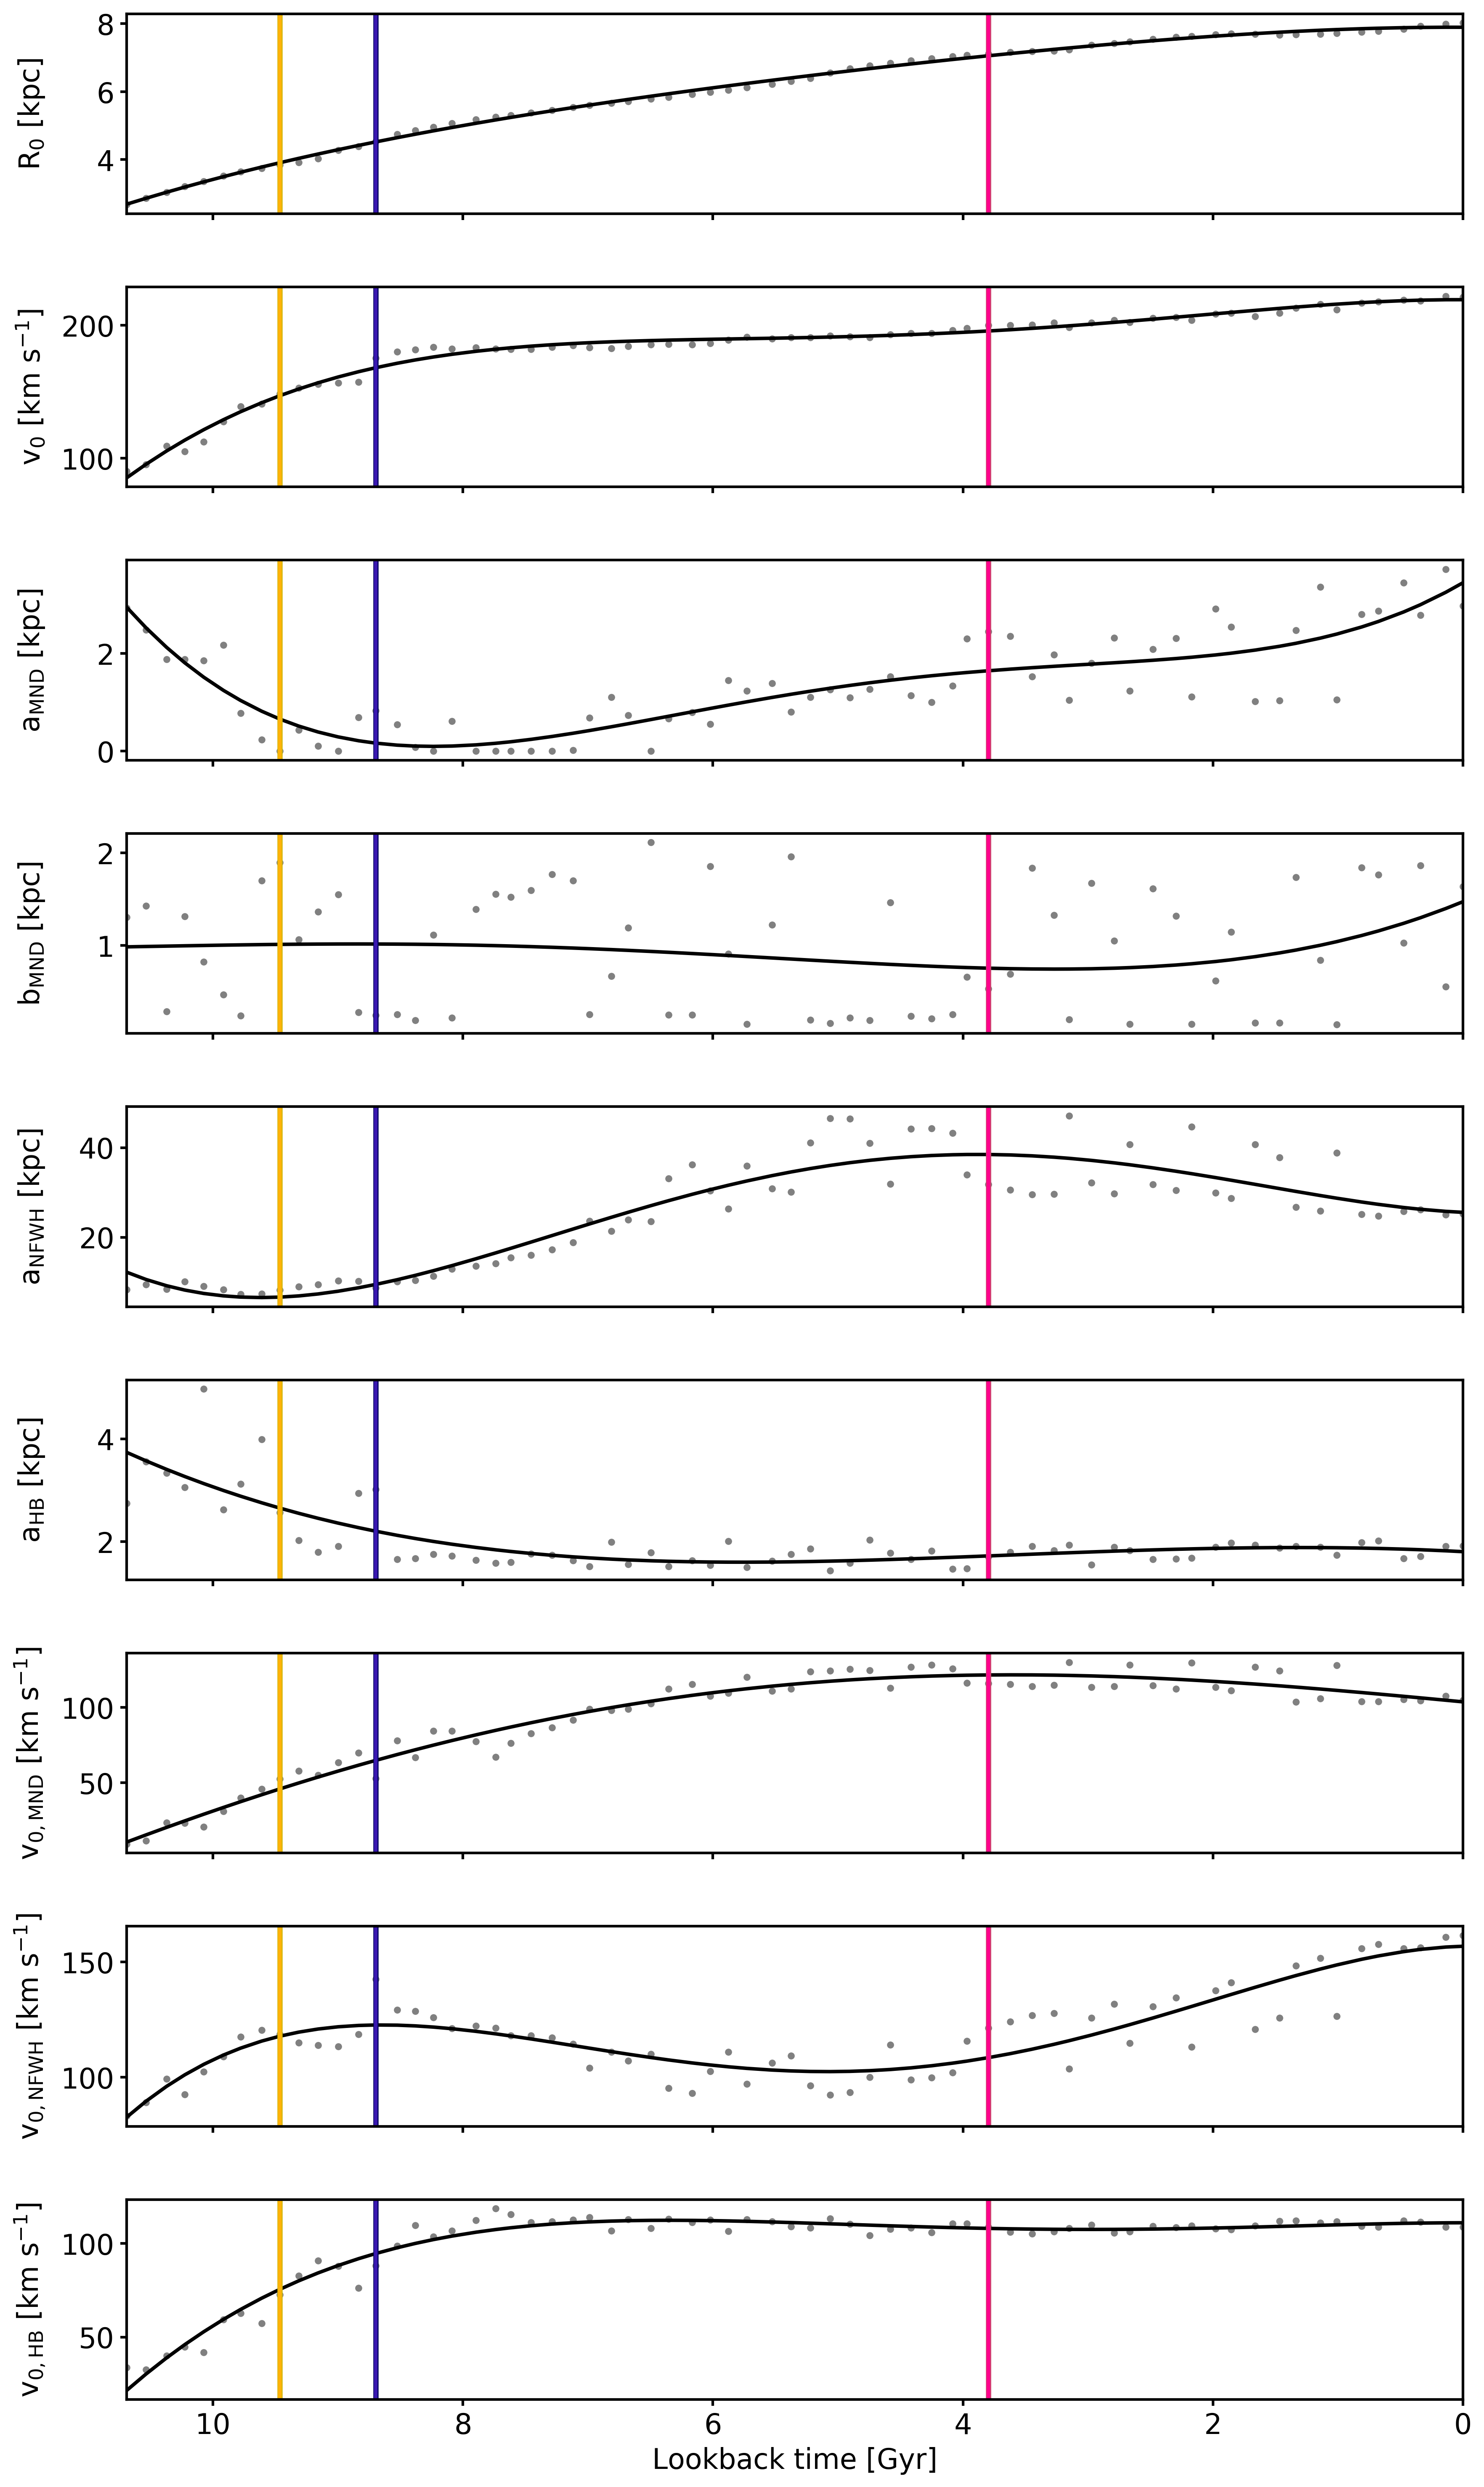
\includegraphics[width=0.7\textwidth]{plots/Auriga/fitted_potential_evolution_dec18.png}
\caption{Evolution of all fit parameters over time. R$_0$ and v$_0$ describe the overall evolution and the other parameters describe scale length - and height, if applicable - and their contribution to the circular velocity. The grey dots are the best fit values and the black lines are polynomial fits of 4th order for each parameter. The vertical lines mark the merger times of the three biggest merger events the main halo galaxy has experiences. The pink merger was the latest and biggest merger while the yellow merger contributed the least mass of these. In the first two panels, we see that the growth of the galaxy is continuous. The second merger flattened out the rise of the total circular velocity which is measured at R$_0$. R$_0$ is set to be a third of the galaxy radius. The spheroid's parameters are very constant since the second merger, while the disk and the \ac{DM} halo are affected by the last merger. While the disk seems to grow in size, its contribution to the total circular velocity decreases. On the contrary, the \ac{DM} halo contracts but it's contribution to the velocity rises more steeply. This shows, that these mergers have a strong impact on the evolution of the potential of this galaxy. Nevertheless, with the fits of the values we can still assume a slowly varying potential which is essential for the action evolution.}\label{fig:pot_val_evol}
\end{figure}
In the potential parameters, we see how the galaxy grows and how the growth is affected by mergers. The indicated mergers are described in more detail in the next Section and in Table \ref{tab:prog_overview}. The overall trend is very smooth and without any outliers. The spheroid remains very constant after the second biggest merger while the other components, especially the disk, have a larger scatter. The latest and biggest merger has a strong impact on the disk and the \ac{DM} halo. The fits of the values allow us to still carry out the action investigations (from Section \ref{subsec:GCs_action_space} on) under the assumption of a slowly varying potential. 

\iffalse
\begin{figure}
\captionsetup{format=plain}
    \centering
    \begin{subfigure}[b]{0.3\textwidth}
	    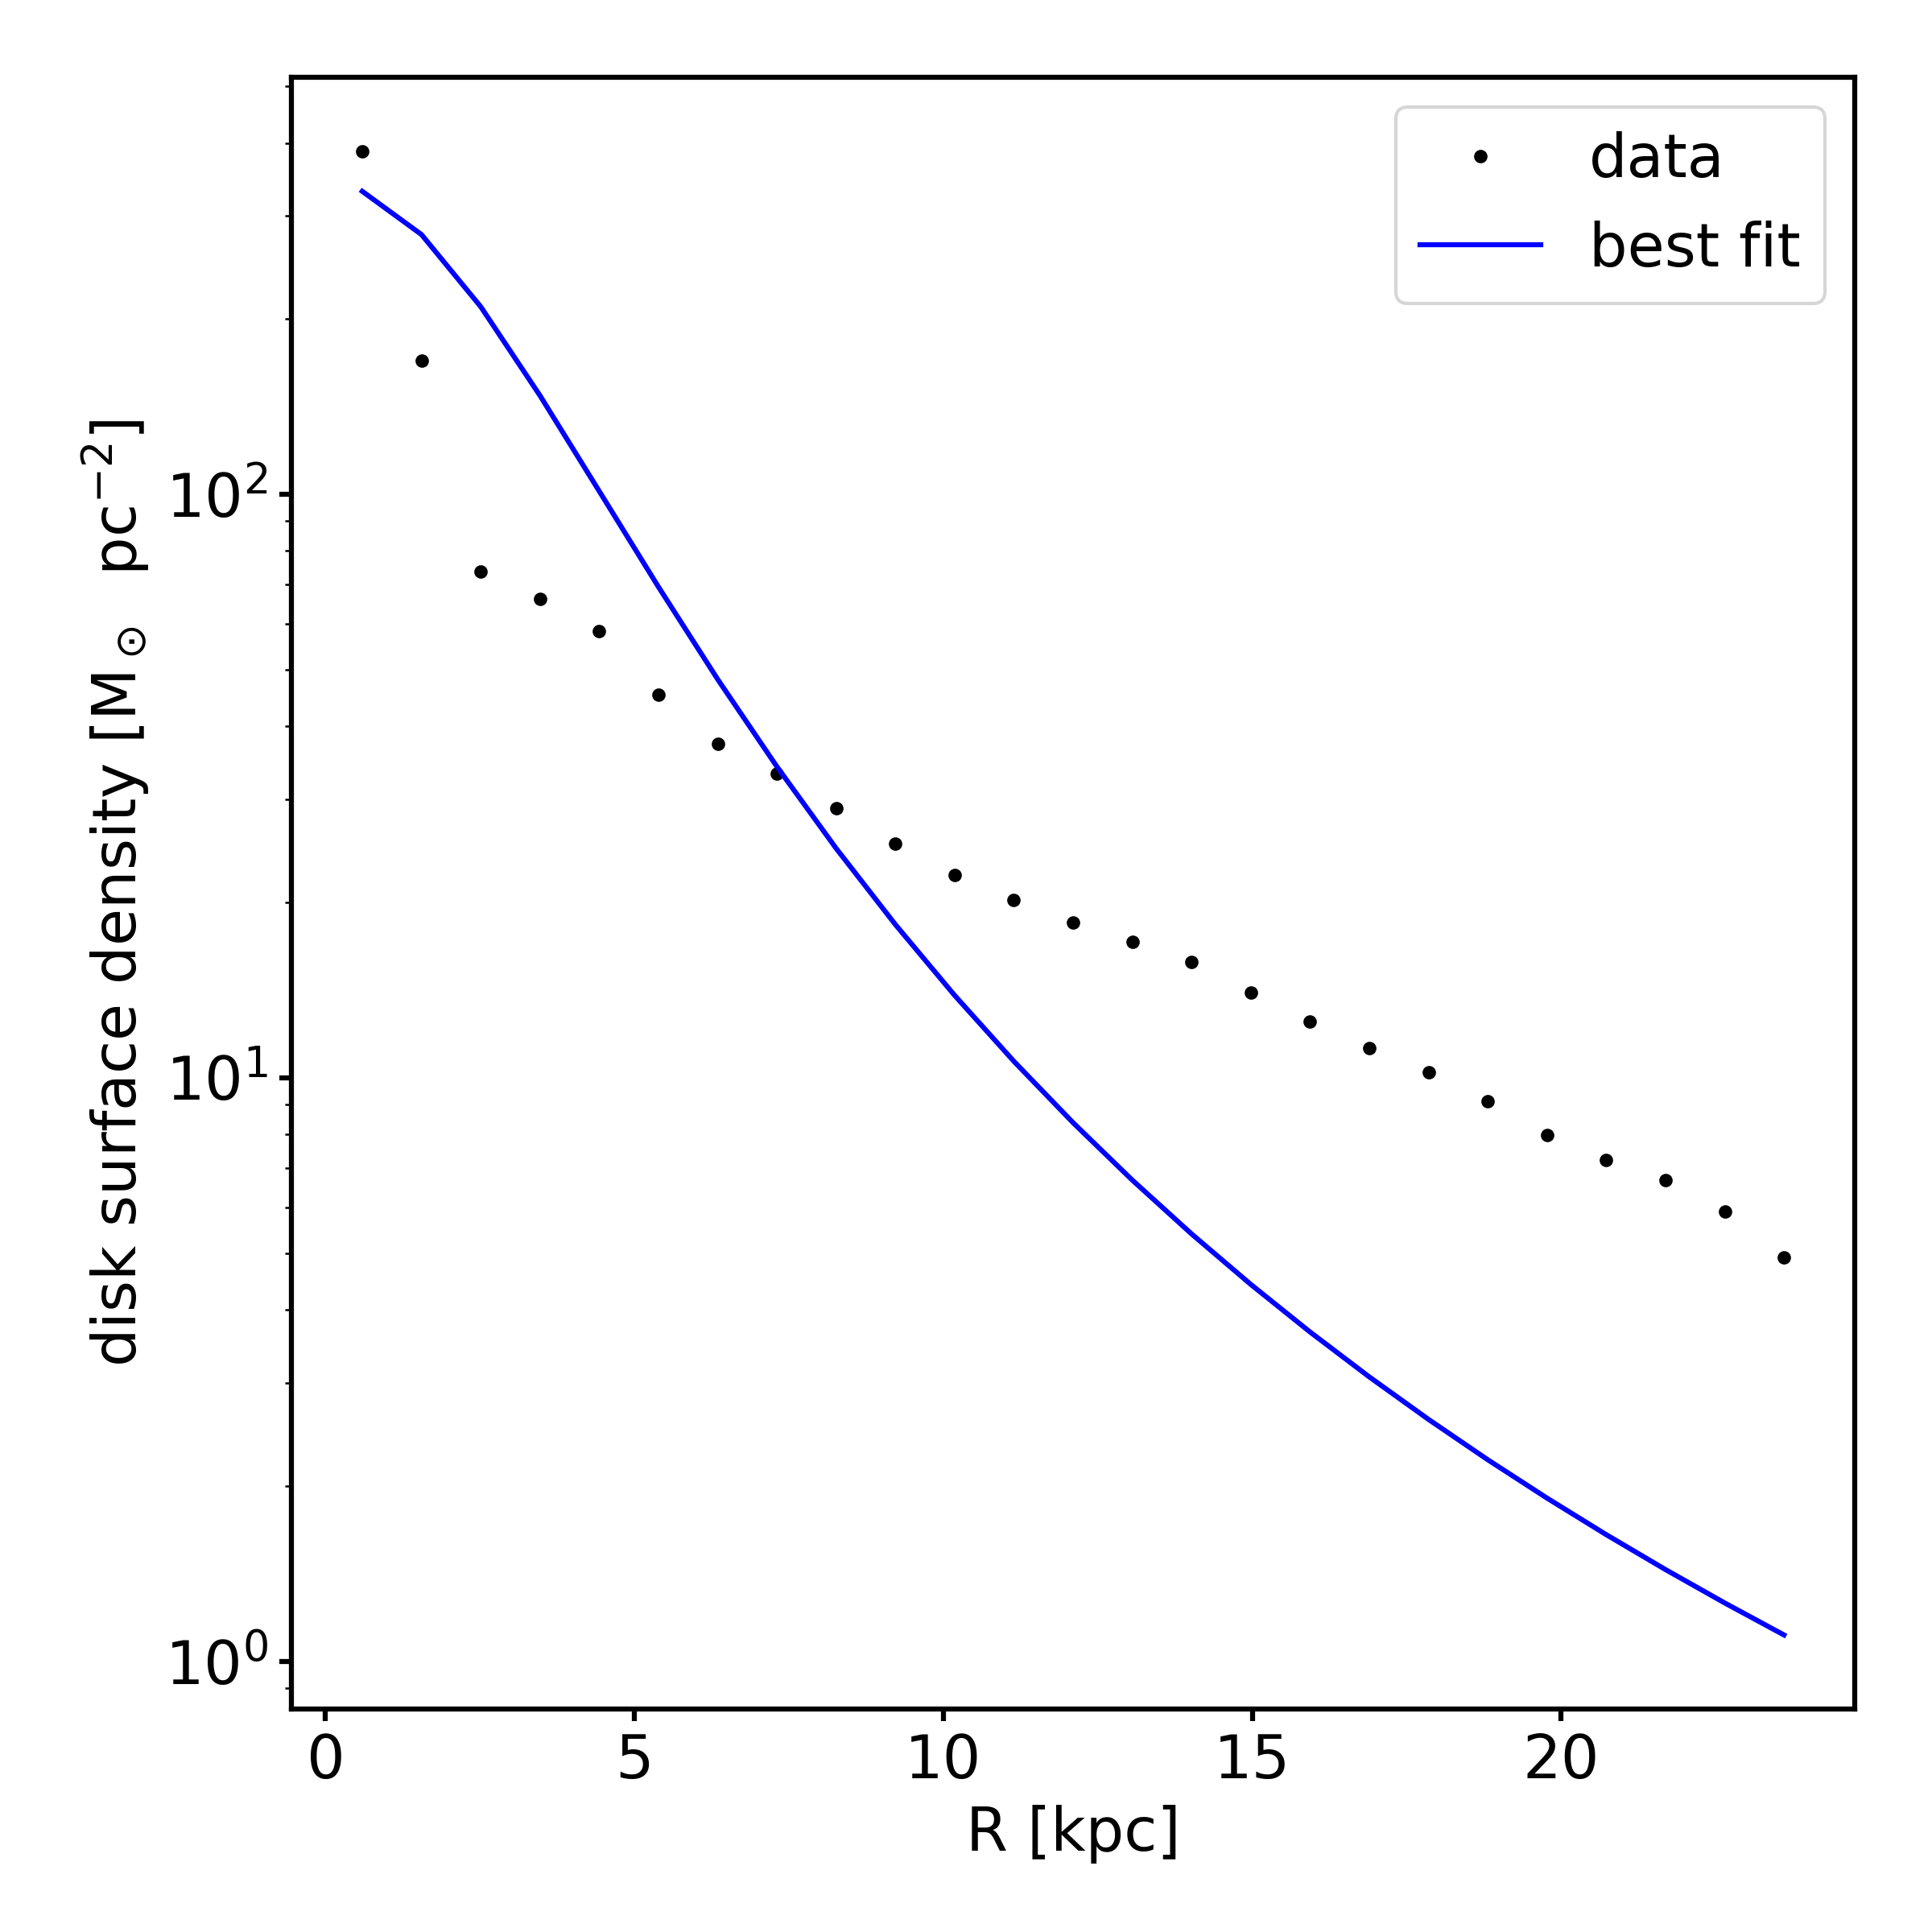
\includegraphics[width=\textwidth]{plots/Auriga/surface_dens_disk_fit_data.png}
	    \label{fig:disk_surfdens_fit}
    \end{subfigure}
    ~ %add desired spacing between images, e. g. ~, \quad, \qquad, \hfill etc. 
      %(or a blank line to force the subfigure onto a new line)
    \begin{subfigure}[b]{0.3\textwidth}
    \centering
    	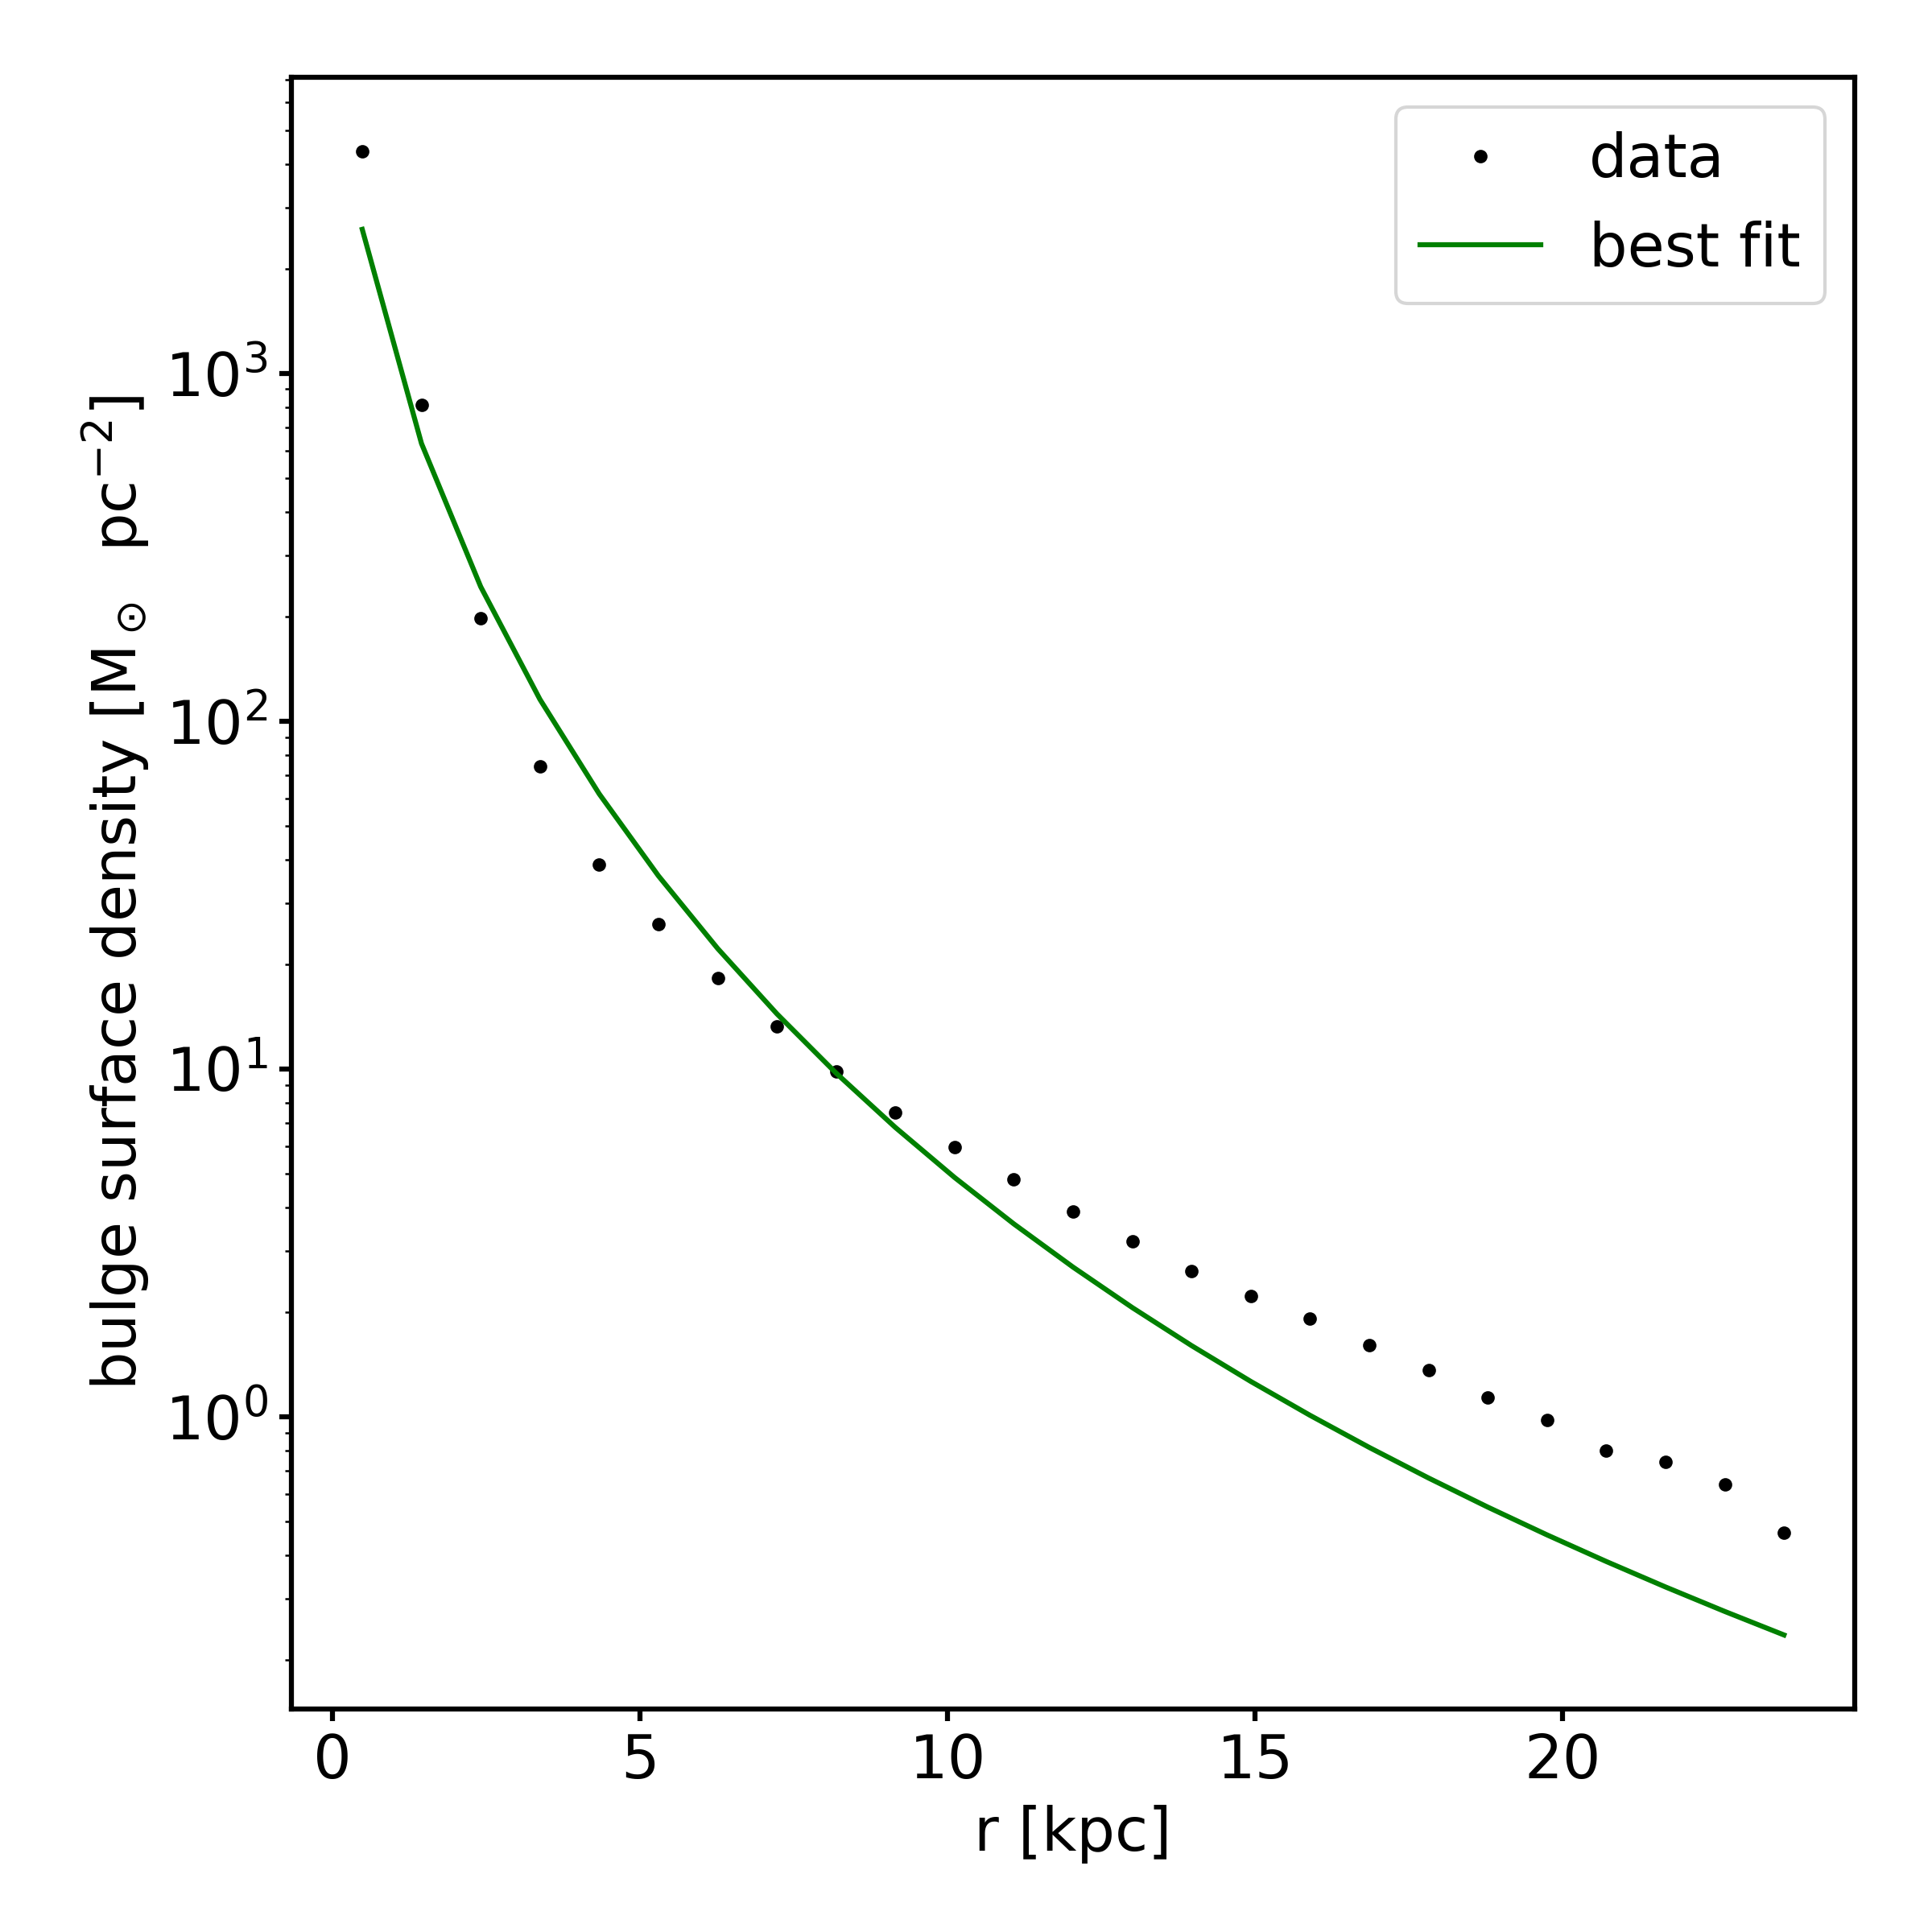
\includegraphics[width=\textwidth]{plots/Auriga/surface_dens_spher_fit_data.png}
    	\label{fig:spher_surfdens_fit}
    \end{subfigure}
    ~ %add desired spacing between images, e. g. ~, \quad, \qquad, \hfill etc. 
    %(or a blank line to force the subfigure onto a new line)
    \begin{subfigure}[b]{0.3\textwidth}
    \centering
    	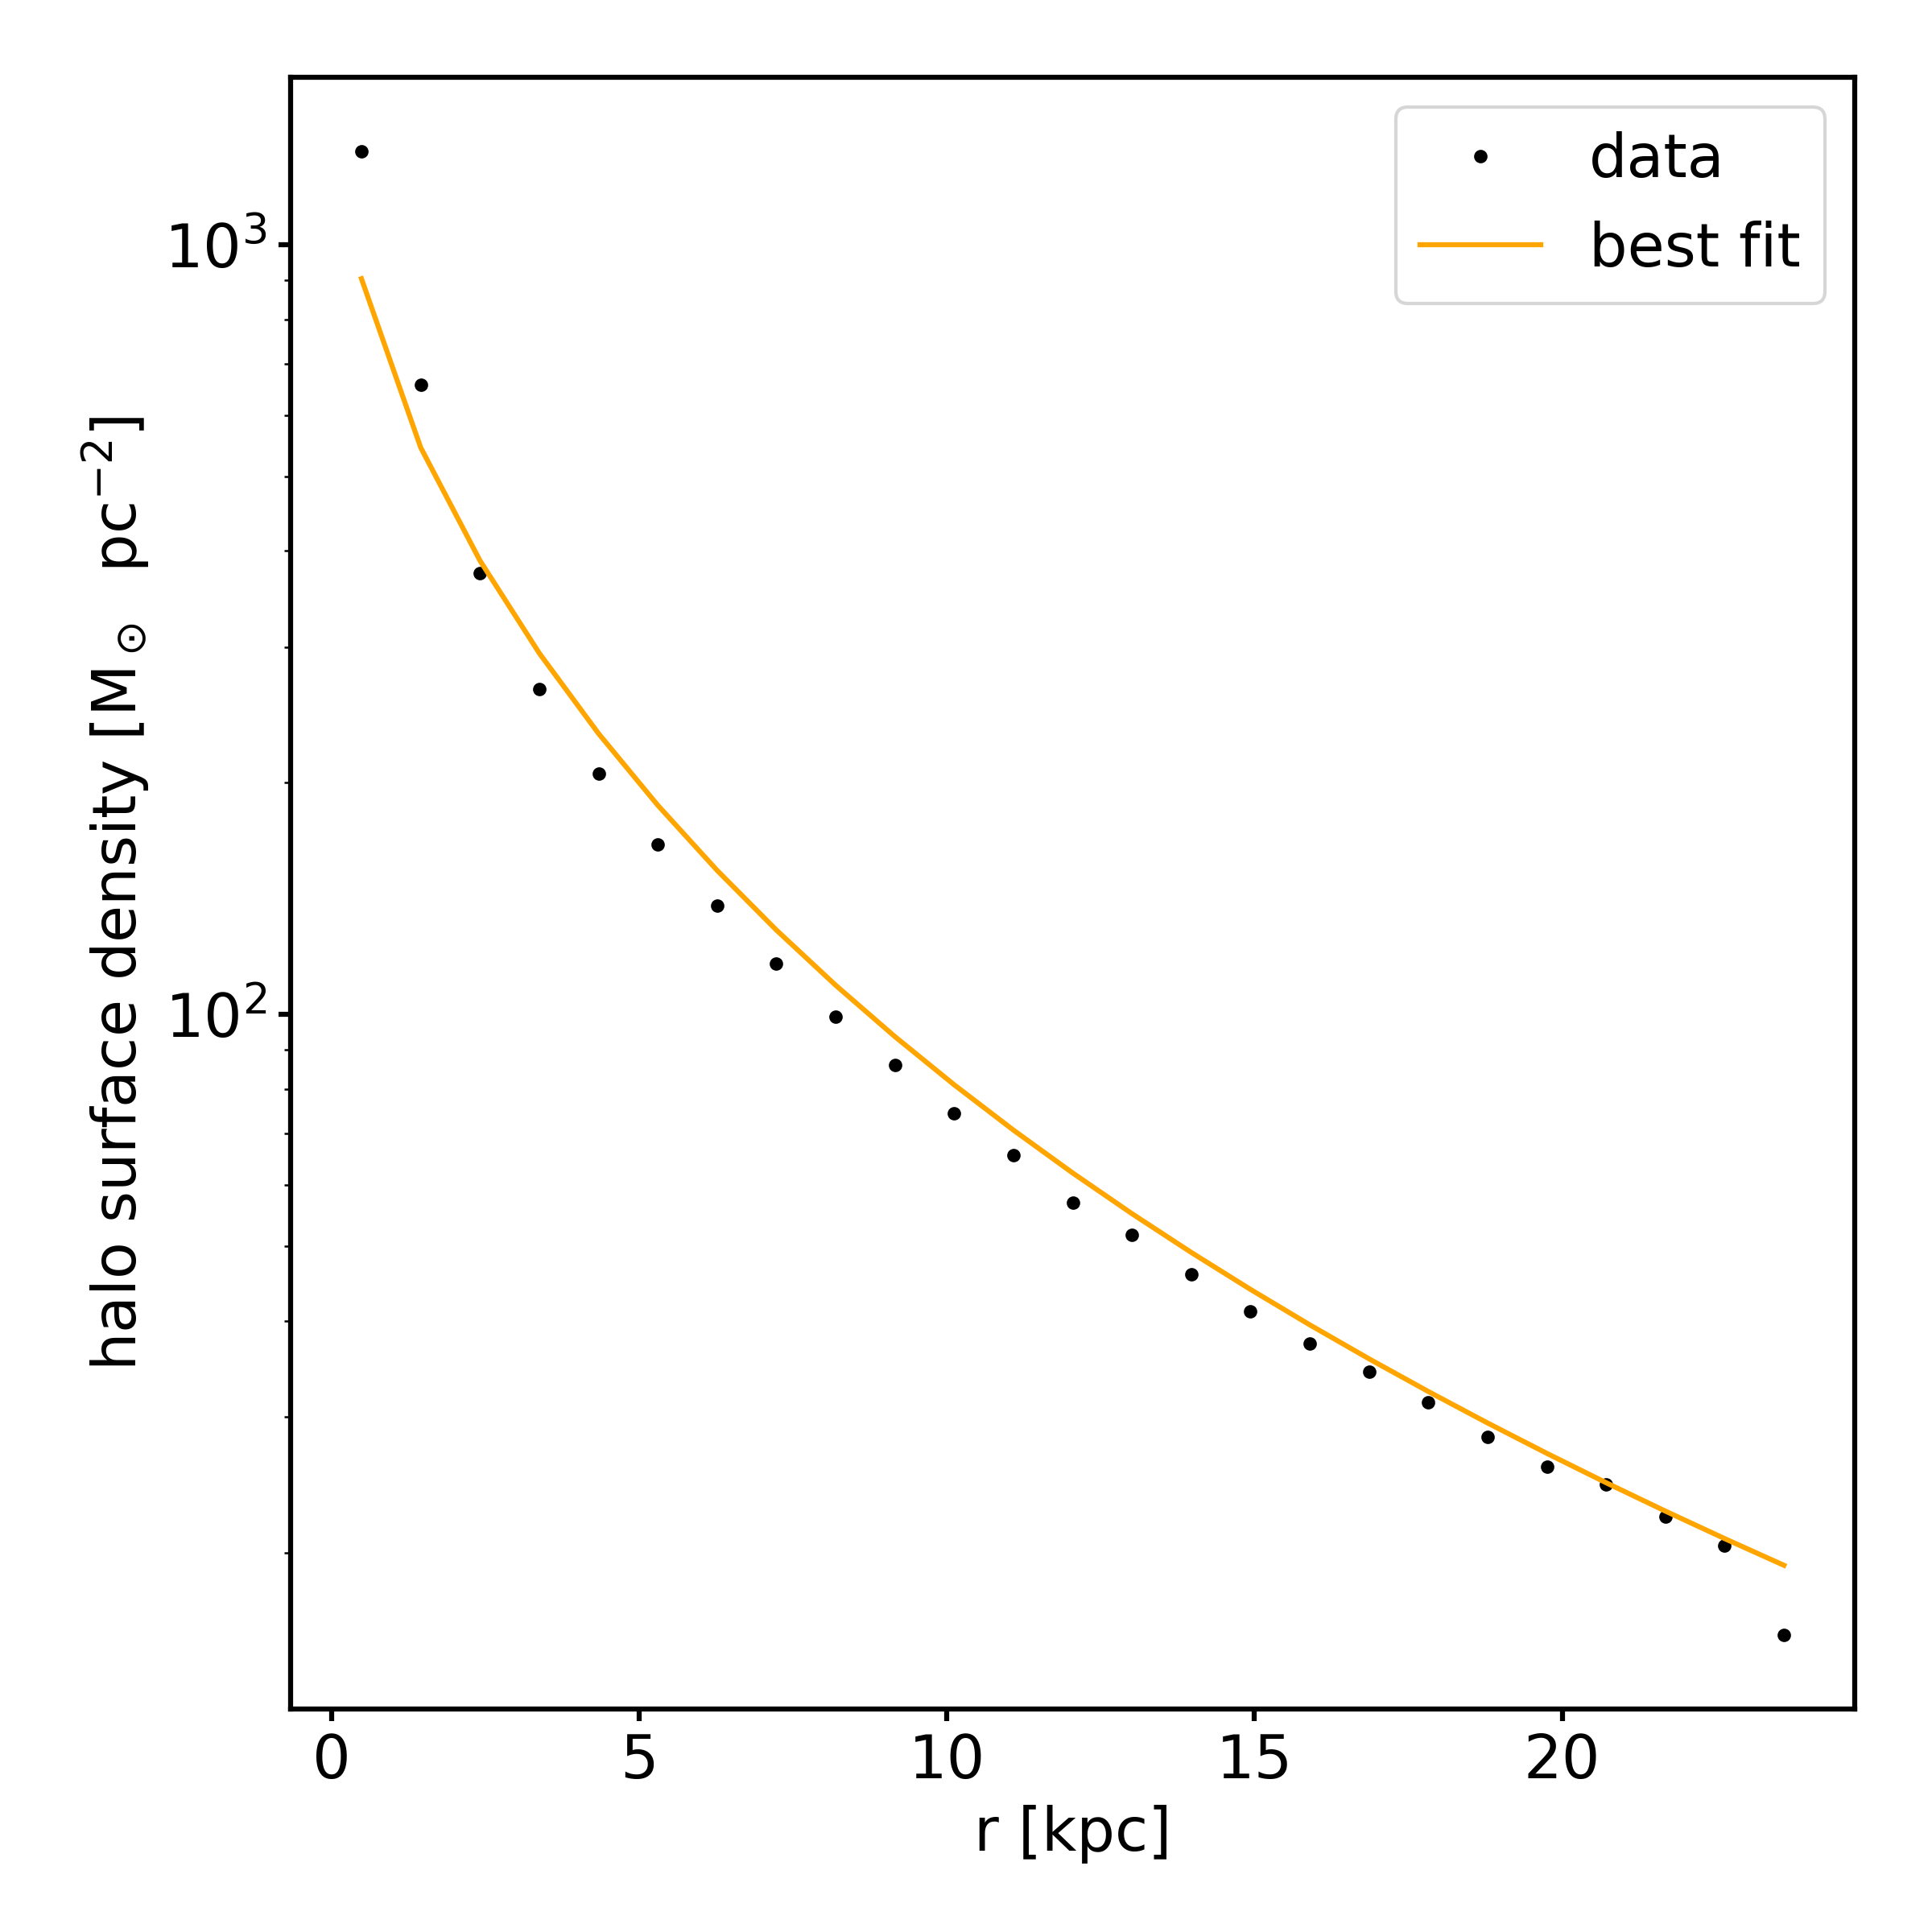
\includegraphics[width=\textwidth]{plots/Auriga/surface_dens_halo_fit_data.png}
    	\label{fig:halo_surfdens_fit}
    \end{subfigure}
    
    \begin{subfigure}[b]{0.3\textwidth}
        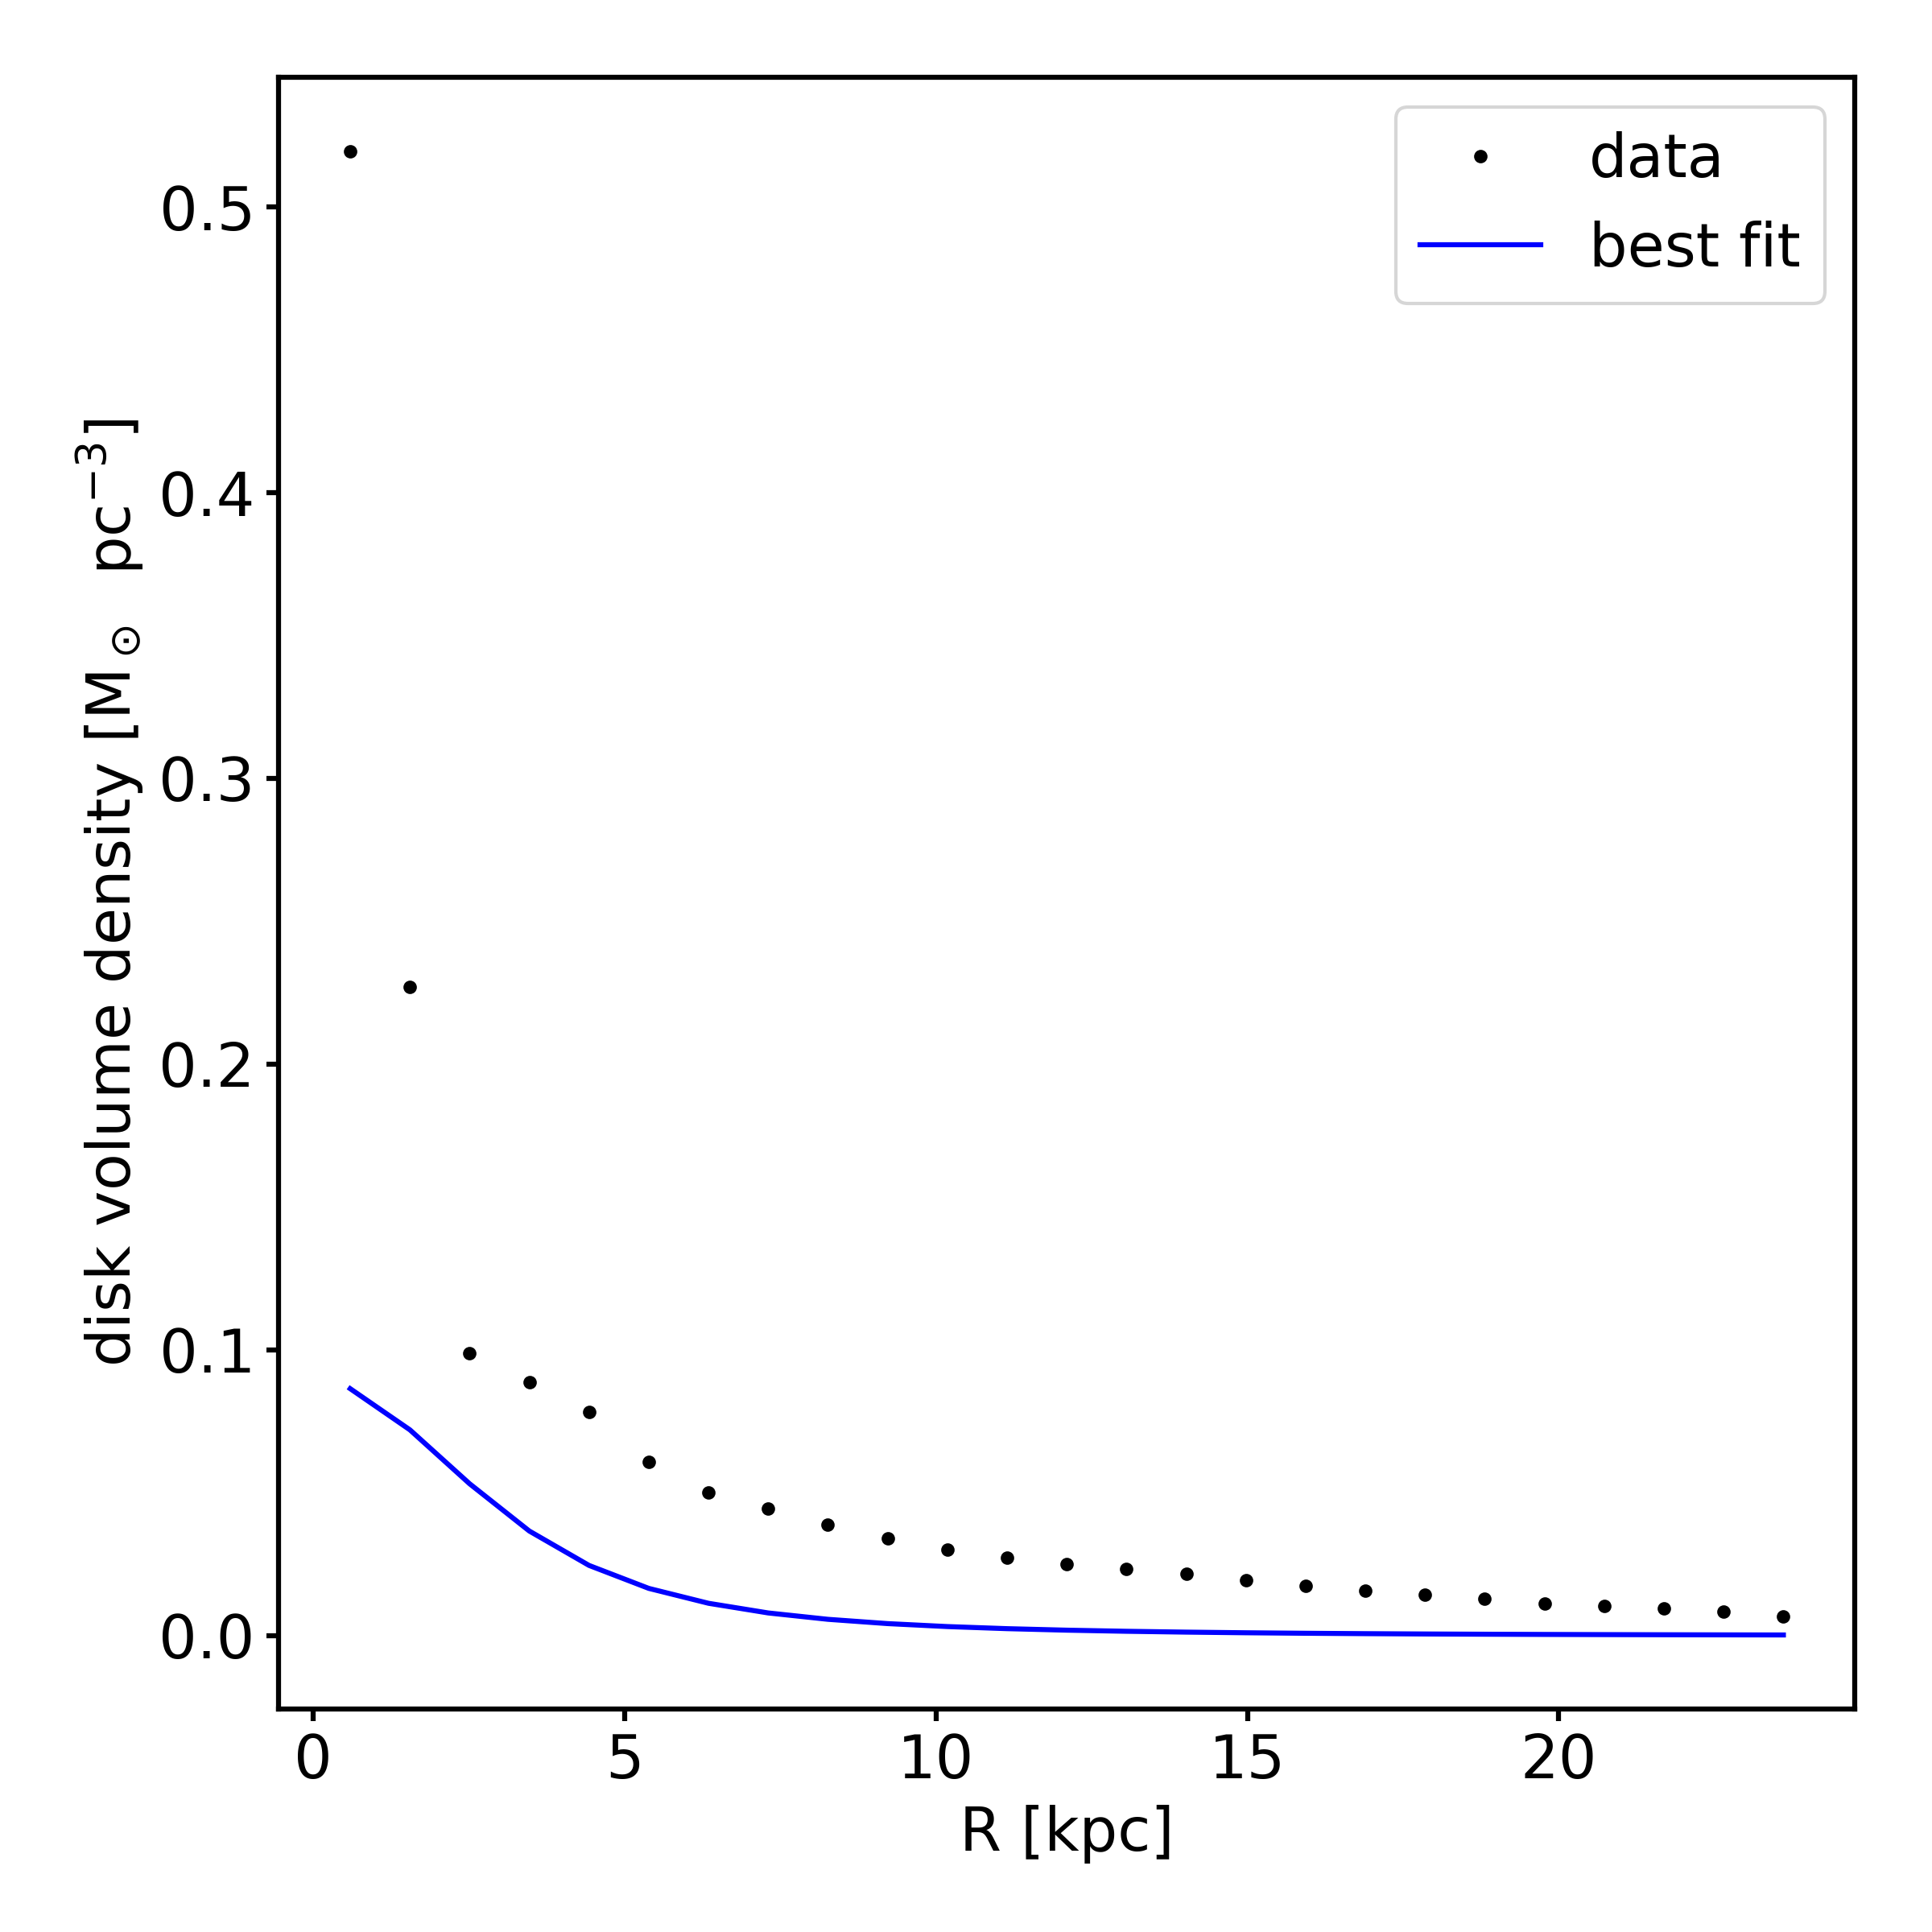
\includegraphics[width=\textwidth]{plots/Auriga/volume_dens_disk_fit_data.png}
	    \label{fig:disk_voldens_fit}
    \end{subfigure}
    ~ %add desired spacing between images, e. g. ~, \quad, \qquad, \hfill etc. 
    %(or a blank line to force the subfigure onto a new line)
    \begin{subfigure}[b]{0.3\textwidth}
    \centering
    	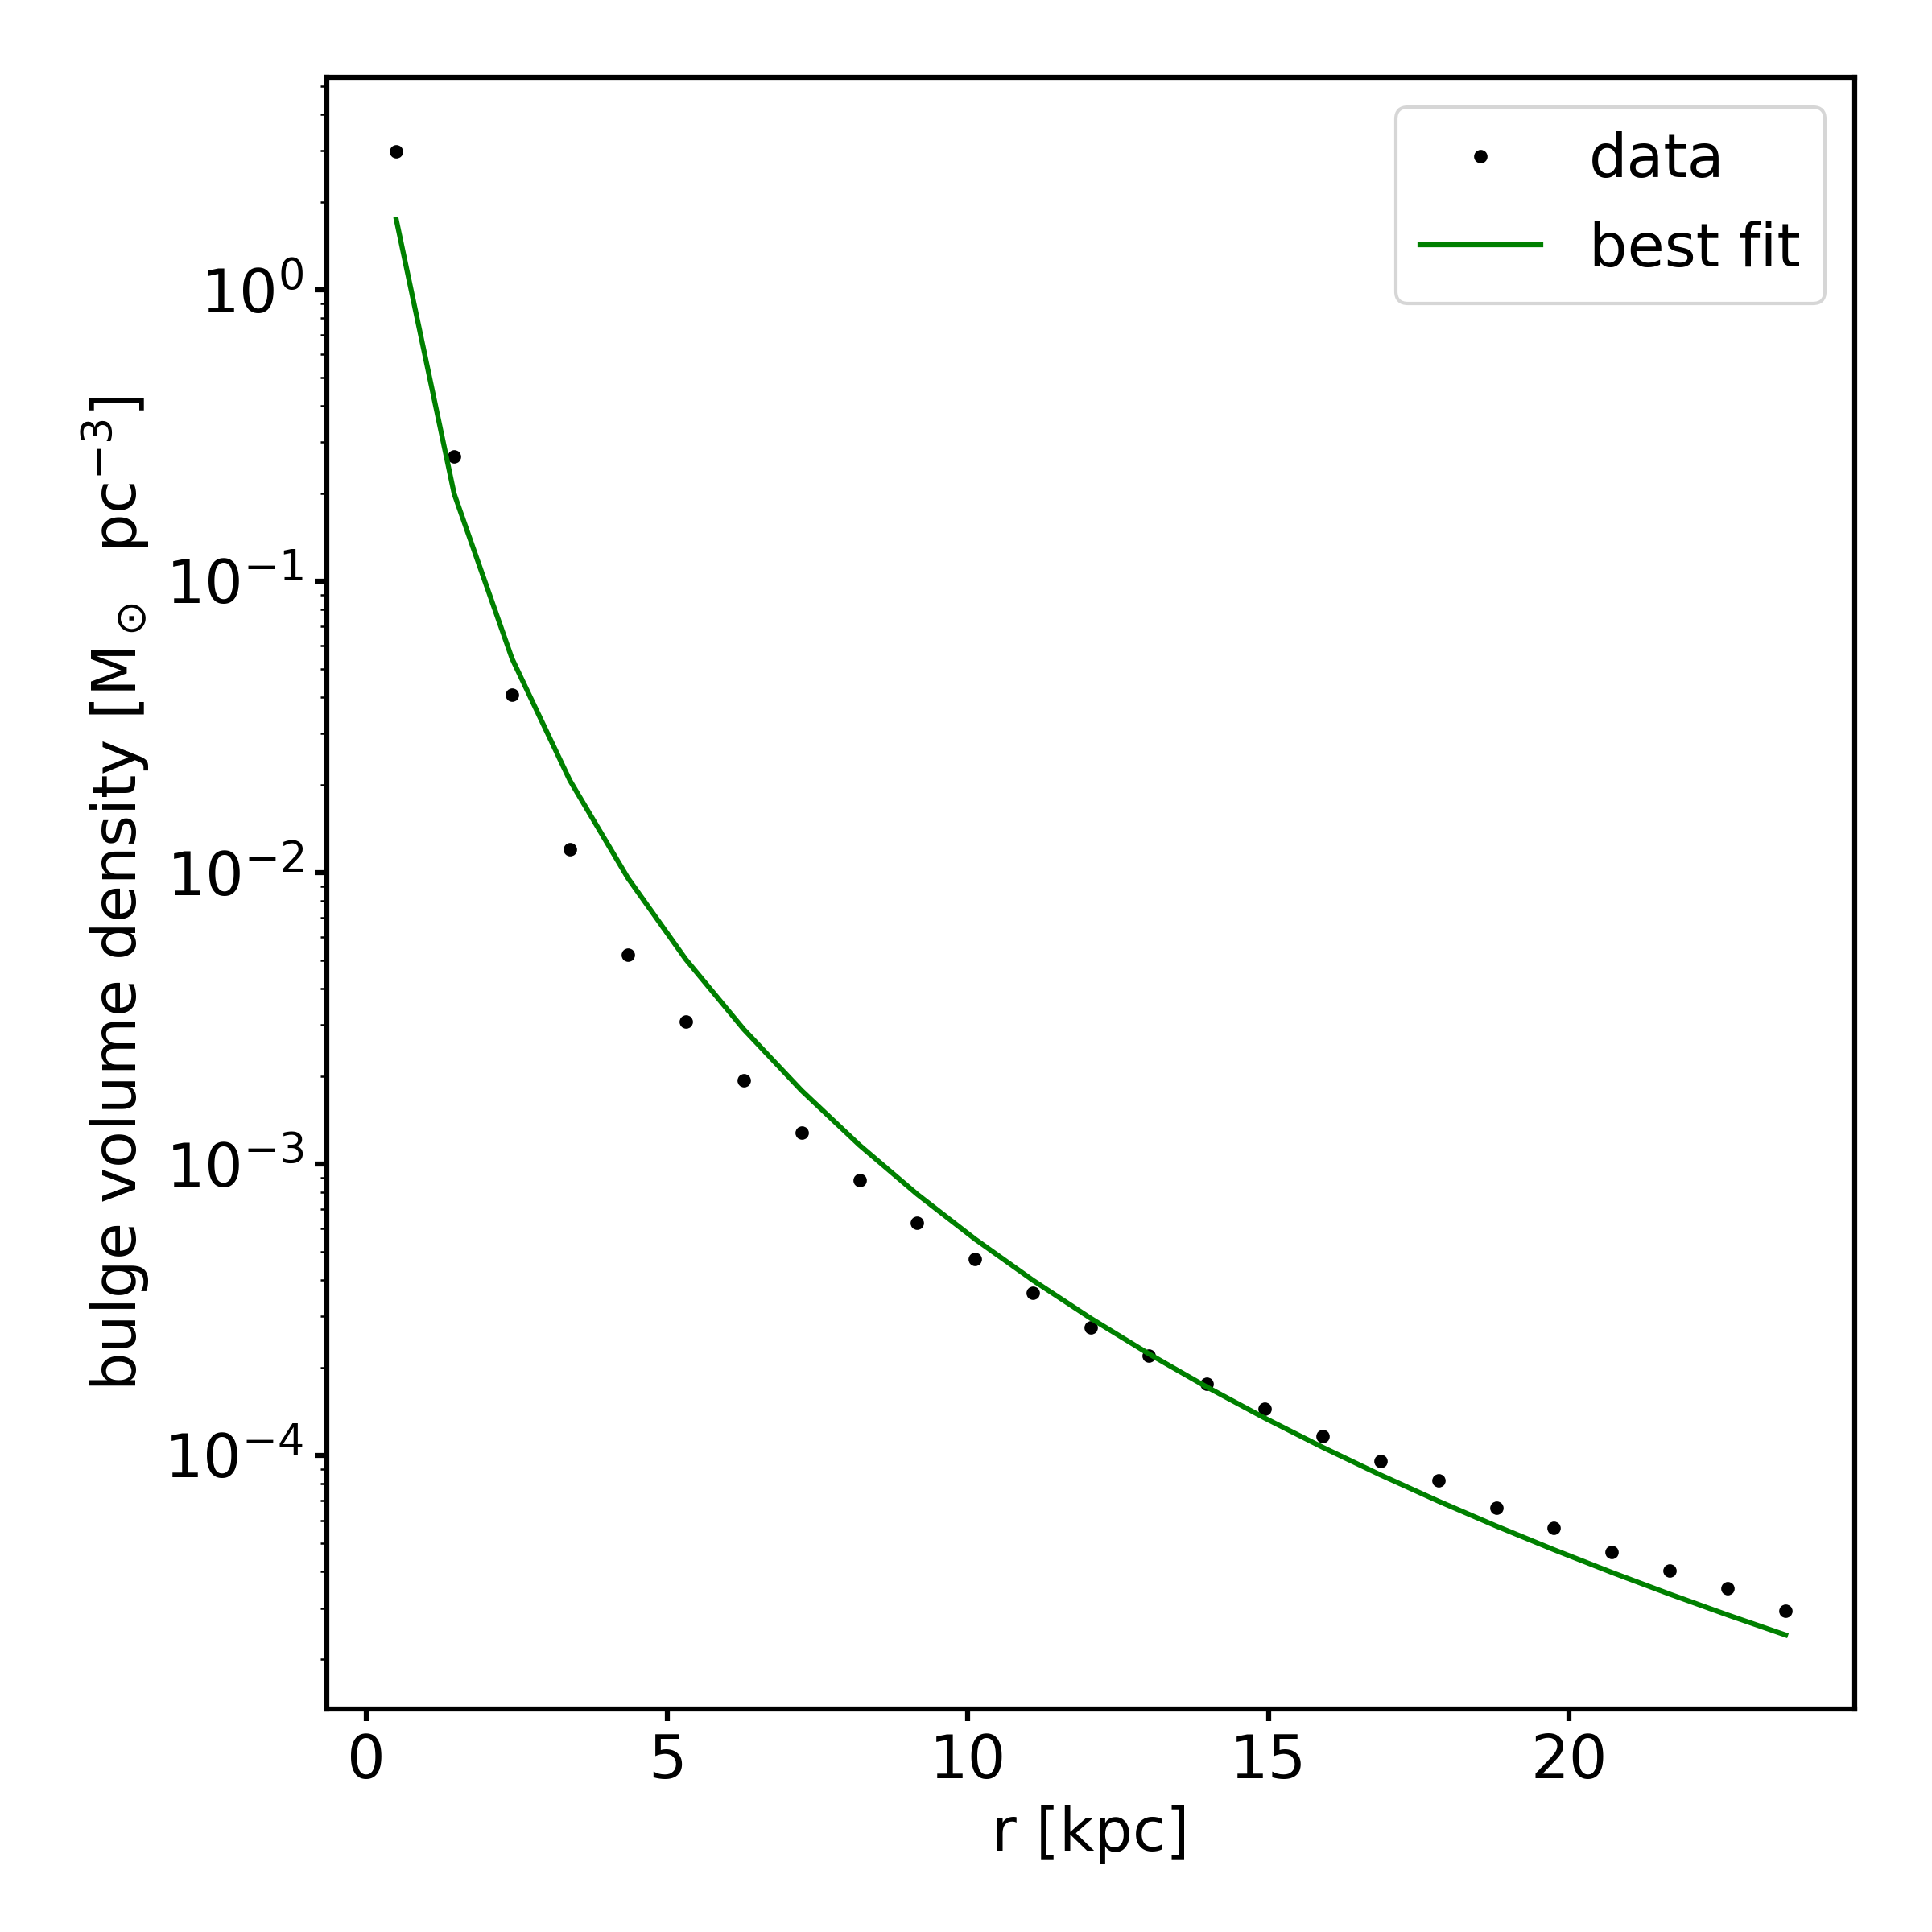
\includegraphics[width=\textwidth]{plots/Auriga/volume_dens_bulge_fit_data.png}
    	\label{fig:spher_voldens_fit}
    \end{subfigure}
    ~ %add desired spacing between images, e. g. ~, \quad, \qquad, \hfill etc. 
    %(or a blank line to force the subfigure onto a new line)
    \begin{subfigure}[b]{0.3\textwidth}
        \centering
    	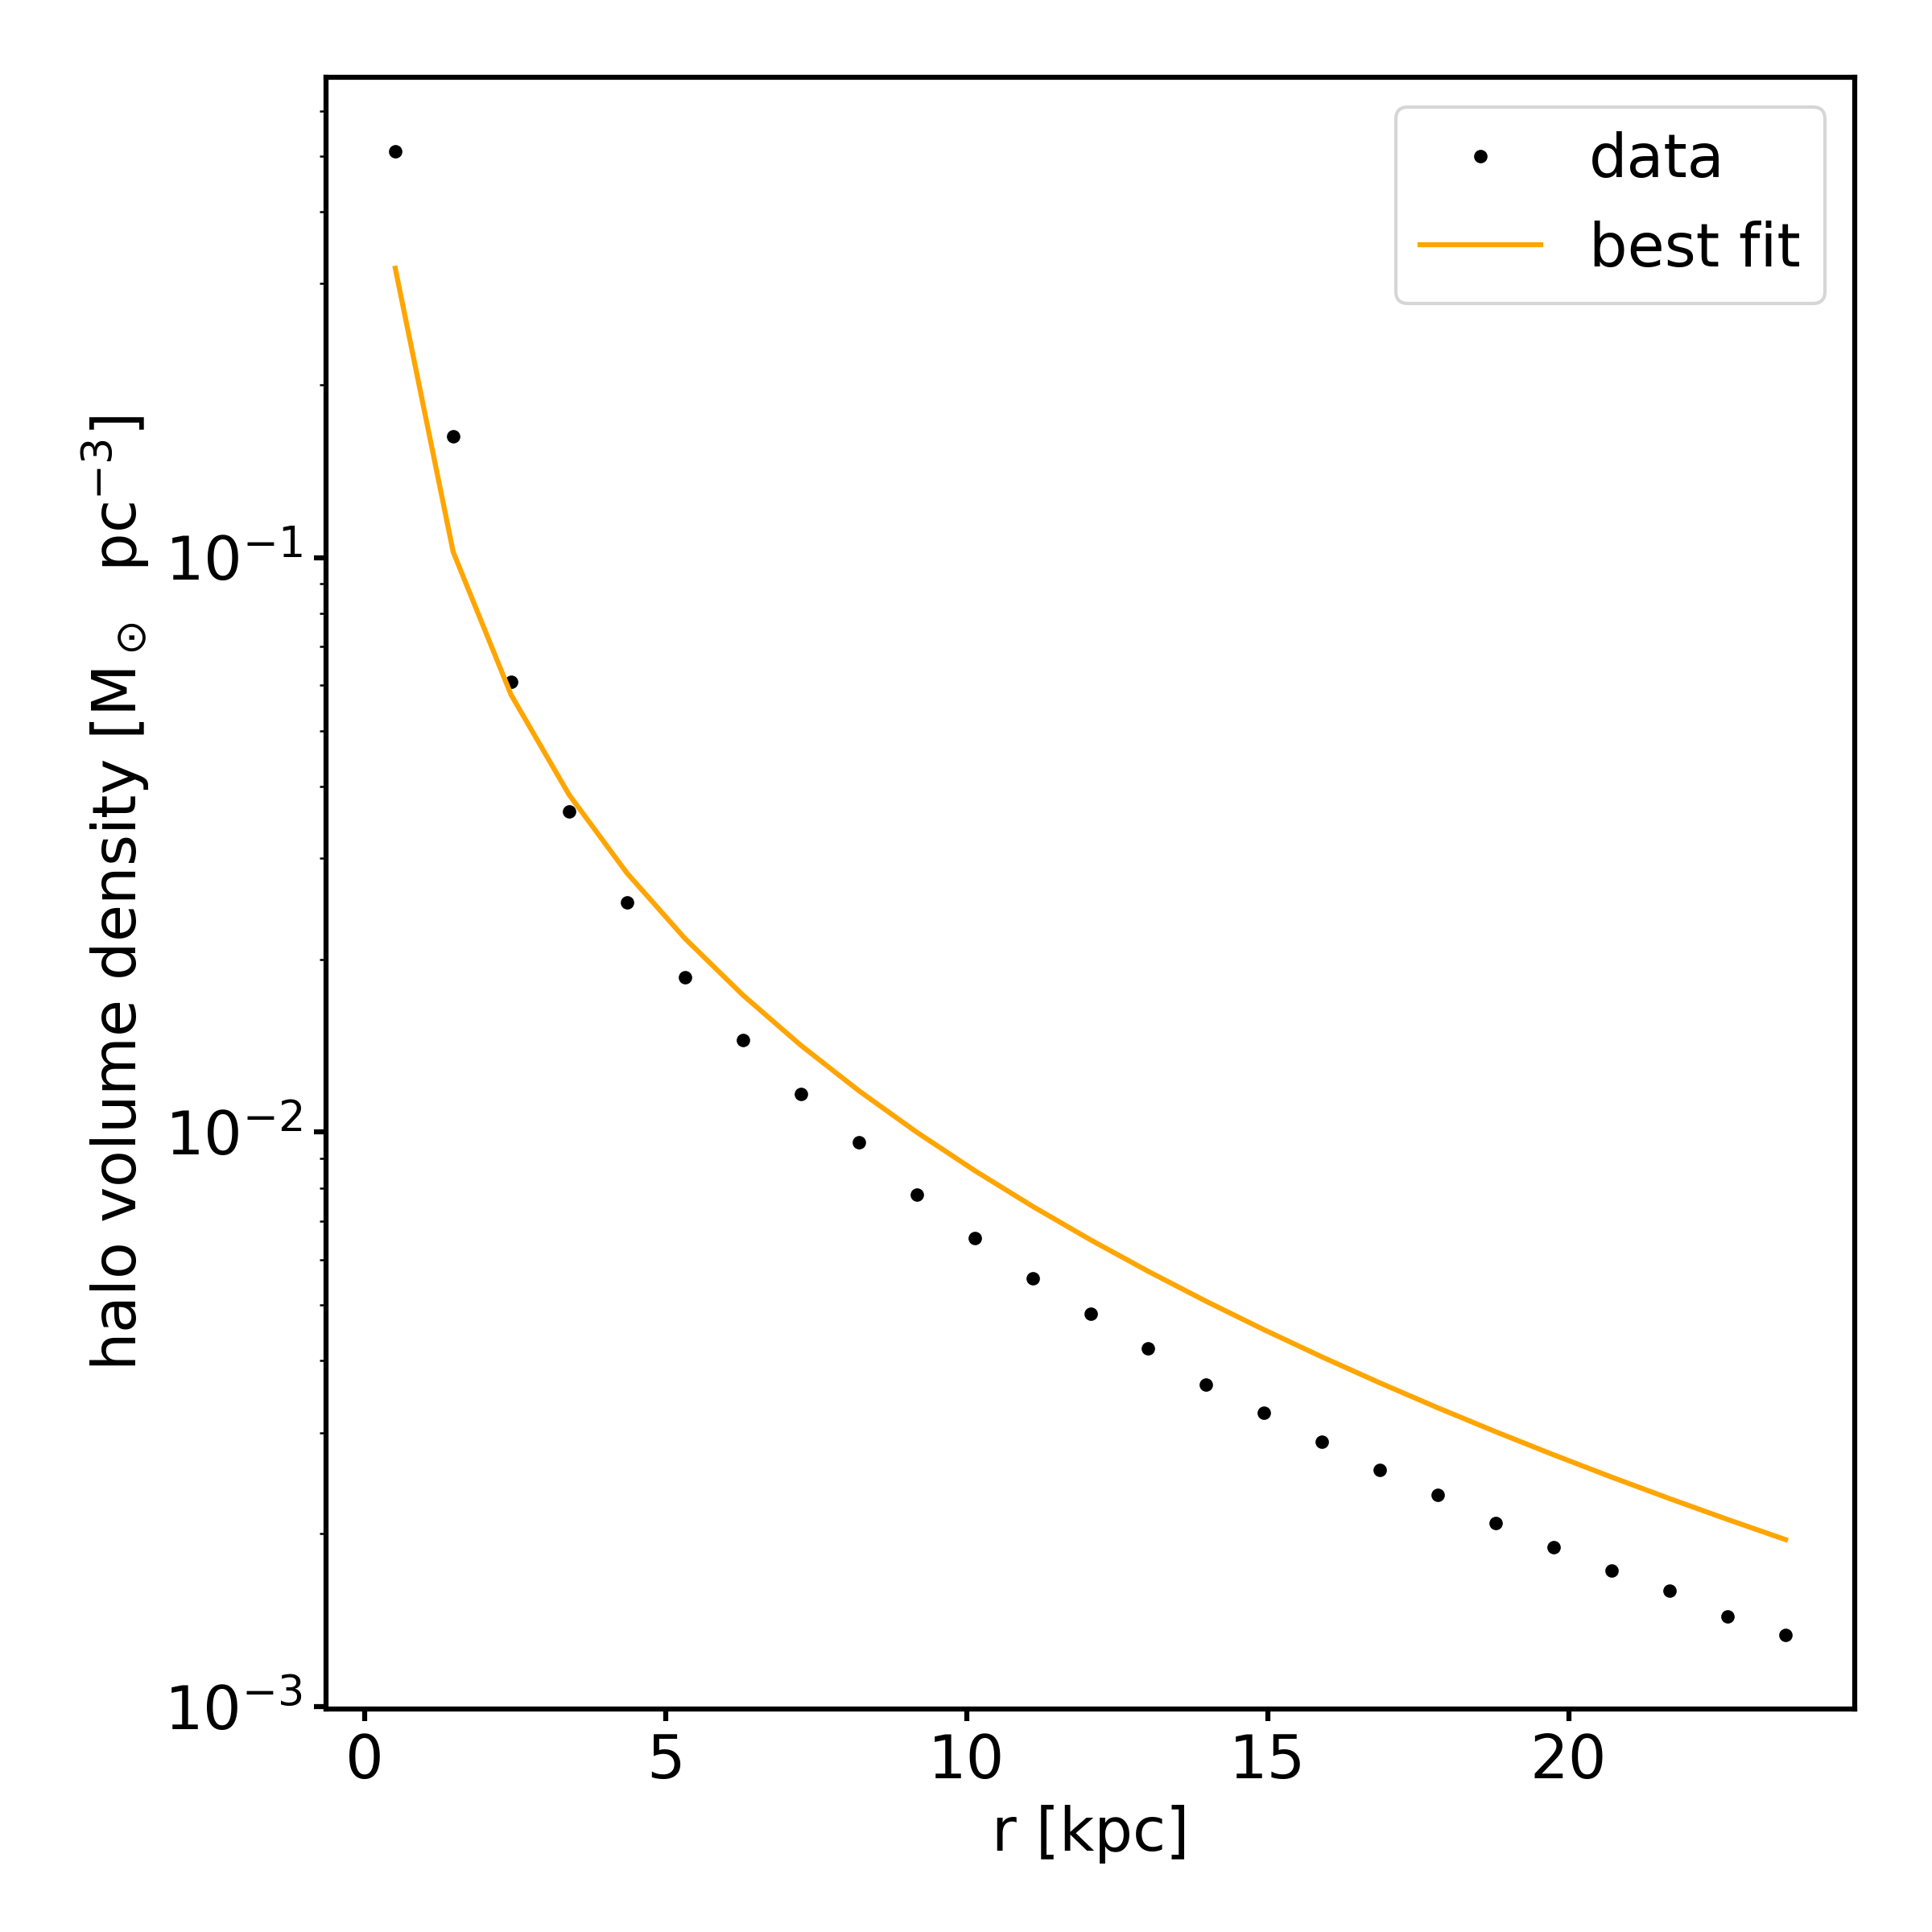
\includegraphics[width=\textwidth]{plots/Auriga/volume_dens_halo_fit_data.png}
	    \label{fig:halo_voldens_fit}
    \end{subfigure}
    \caption{Surface densities (upper row) and mass densities (lower row) of the components and their best fits at $\textit{z}=0$. Left (blue): stellar disk, middle (green): stellar spheroid, right (yellow): \ac{DM} halo.}\label{fig:single_pot_fits}
\end{figure}
\fi
\\
\begin{figure}[htbp]
\captionsetup{format=plain}
\centering
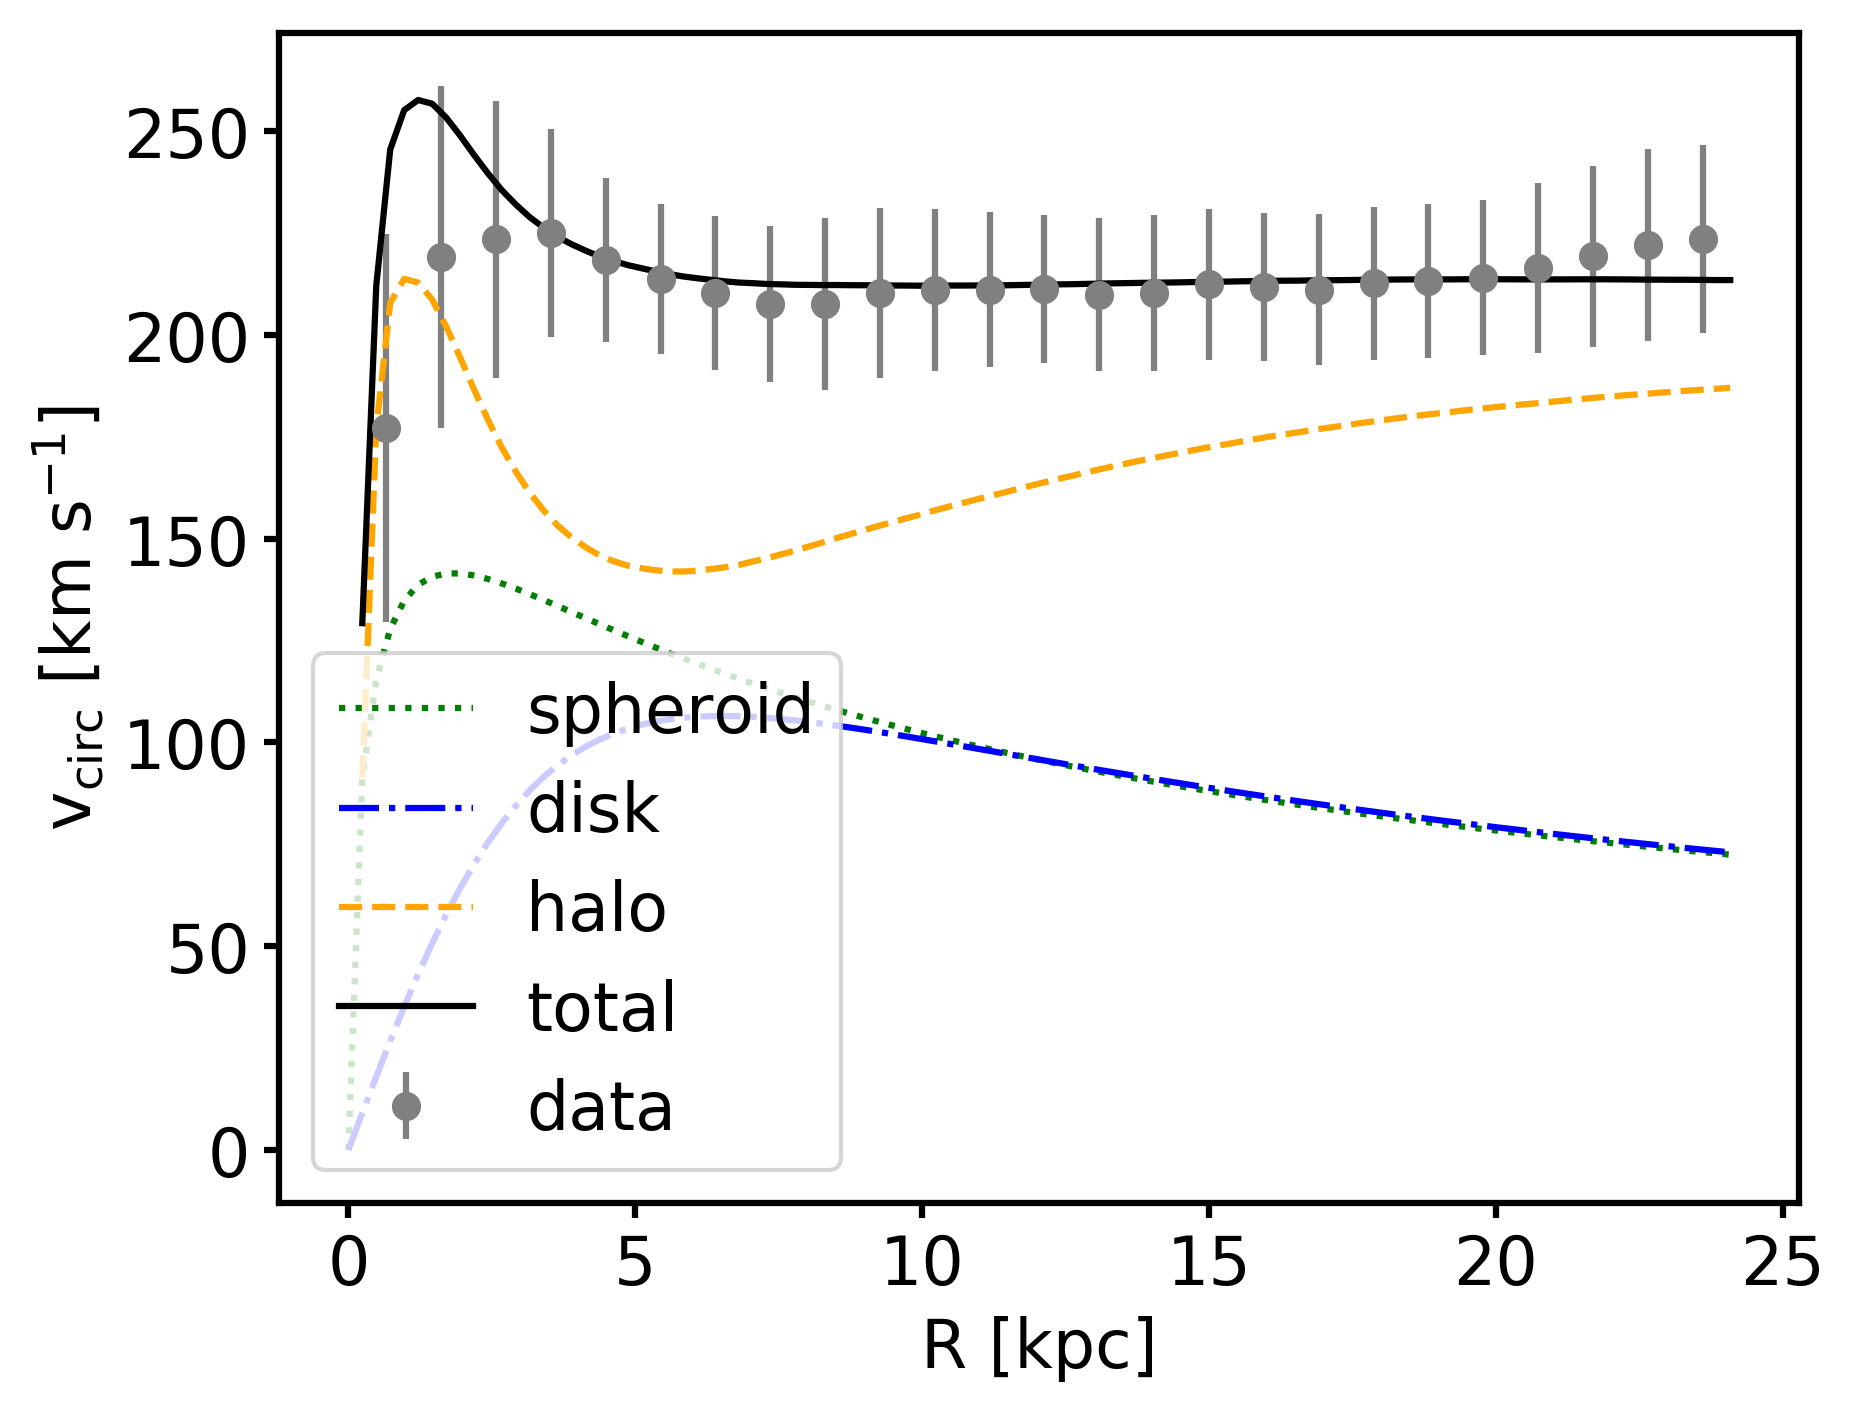
\includegraphics[width=0.8\textwidth]{plots/Auriga/best_fit_circular_velocity_via_formula_snap_127.png}
\caption{Circular velocity at \textit{z} = 0: data (grey circles), total (black solid line), disk (blue dashed dotted line), bulge (green dotted line) and halo (orange). The data is the mean tangential velocity of all stars which have $\epsilon > 0.95$. The other components and the total distribution are calculated analytically. The total curve matches the data within its errors. Disk and spheroid overlay in the outer parts which is due to the decomposition where their proportion is nearly $1:1$. The \ac{DM} distribution has a peak in the center. This is probably due to an underestimation of the spheroid component in the center which we can see find in the density fit in Figure \ref{fig:spheroid_fit}. In the outer parts (R$>\mathrm{R}_0$), the curves behave as they are expected to do.}. \label{fig:circ_vel_fit}
\end{figure}
\\To verify the goodness of the total potential, we show the circular velocity curve in Figure \ref{fig:circ_vel_fit}. While in the innermost part the \ac{DM} proportion might be too high due to an underestimation of the stellar spheroid, the \ac{DM} proportion in the outer part seems correct. The disk is underestimated due to the sharp decomposition. In overall, the total circular velocity matches the data and the fit in the outer parts, where the particles we investigate in Section \ref{sec:Dynamics} are, is reliable.  

\subsection{What not to do when fitting a gravitational potential}\label{subsec:wrong_pot_fit}
\subsubsection{Fit the potential in one step}
In the first Ansatz, we also worked with the three component analytic potential but we assumed that we can just fit the combined potential to the 'pot' value of a different amount of random particles (up to 1 million) of the simulation data. It resulted in an overestimation of the 



\subsubsection{Choosing too simple fitting routines}




\textbf{Put in table with parameter comparison }